%% Run LaTeX on this file several times to get Table of Contents,
%% cross-references, and citations.

\documentclass[11pt]{book}
\usepackage{gvv-book}
\usepackage{gvv}
\usepackage{caption}
%\usepackage{amsmath}
%\usepackage{Wiley-AuthoringTemplate}
\usepackage[sectionbib,authoryear]{natbib}% for name-date citation comment the below line
%\usepackage[sectionbib,numbers]{natbib}% for numbered citation comment the above line
\usepackage{natbib}
%%********************************************************************%%
%%       How many levels of section head would you like numbered?     %%
%% 0= no section numbers, 1= section, 2= subsection, 3= subsubsection %%
\setcounter{secnumdepth}{3}
%%********************************************************************%%
%%**********************************************************************%%
%%     How many levels of section head would you like to appear in the  %%
%%				Table of Contents?			%%
%% 0= chapter, 1= section, 2= subsection, 3= subsubsection titles.	%%
\setcounter{tocdepth}{2}
%%**********************************************************************%%

%\includeonly{ch01}
\makeindex

\begin{document}

\frontmatter
%%%%%%%%%%%%%%%%%%%%%%%%%%%%%%%%%%%%%%%%%%%%%%%%%%%%%%%%%%%%%%%%
%% Title Pages
%% Wiley will provide title and copyright page, but you can make
%% your own titlepages if you'd like anyway
%% Setting up title pages, type in the appropriate names here:
\booktitle{NAVIC L5 POC}

\subtitle{Through C}

\AuAff{G. V. V. Sharma}


%% \\ will start a new line.
%% You may add \affil{} for affiliation, ie,
%\authors{Robert M. Groves\\
%\affil{Universitat de les Illes Balears}
%Floyd J. Fowler, Jr.\\
%\affil{University of New Mexico}
%}

%% Print Half Title and Title Page:
%\halftitlepage
\titlepage

%%%%%%%%%%%%%%%%%%%%%%%%%%%%%%%%%%%%%%%%%%%%%%%%%%%%%%%%%%%%%%%%
%% Copyright Page

\begin{copyrightpage}{2023}
%Title, etc
\end{copyrightpage}

% Note, you must use \ to start indented lines, ie,
% 
% \begin{copyrightpage}{2004}
% Survey Methodology / Robert M. Groves . . . [et al.].
% \       p. cm.---(Wiley series in survey methodology)
% \    ``Wiley-Interscience."
% \    Includes bibliographical references and index.
% \    ISBN 0-471-48348-6 (pbk.)
% \    1. Surveys---Methodology.  2. Social 
% \  sciences---Research---Statistical methods.  I. Groves, Robert M.  II. %
% Series.\\

% HA31.2.S873 2004
% 001.4'33---dc22                                             2004044064
% \end{copyrightpage}

%%%%%%%%%%%%%%%%%%%%%%%%%%%%%%%%%%%%%%%%%%%%%%%%%%%%%%%%%%%%%%%%
%% Only Dedication (optional) 

%\dedication{To my parents}

\tableofcontents
\listoffigures %optional

%\listoffigures %optional
%\listoftables  %optional

%% or Contributor Page for edited books
%% before \tableofcontents

%%%%%%%%%%%%%%%%%%%%%%%%%%%%%%%%%%%%%%%%%%%%%%%%%%%%%%%%%%%%%%%%
%  Contributors Page for Edited Book
%%%%%%%%%%%%%%%%%%%%%%%%%%%%%%%%%%%%%%%%%%%%%%%%%%%%%%%%%%%%%%%%

% If your book has chapters written by different authors,
% you'll need a Contributors page.

% Use \begin{contributors}...\end{contributors} and
% then enter each author with the \name{} command, followed
% by the affiliation information.

% \begin{contributors}
% \name{Masayki Abe,} Fujitsu Laboratories Ltd., Fujitsu Limited, Atsugi, Japan
%
% \name{L. A. Akers,} Center for Solid State Electronics Research, Arizona State University, Tempe, Arizona
%
% \name{G. H. Bernstein,} Department of Electrical and Computer Engineering, University of Notre Dame, Notre Dame, South Bend, Indiana; formerly of
% Center for Solid State Electronics Research, Arizona
% State University, Tempe, Arizona 
% \end{contributors}

%%%%%%%%%%%%%%%%%%%%%%%%%%%%%%%%%%%%%%%%%%%%%%%%%%%%%%%%%%%%%%%%
% Optional Foreword:

%\begin{foreword}
%\lipsum[1-2]
%\end{foreword}

%%%%%%%%%%%%%%%%%%%%%%%%%%%%%%%%%%%%%%%%%%%%%%%%%%%%%%%%%%%%%%%%
% Optional Preface:

%\begin{preface}
%\lipsum[1-1]
%\prefaceauthor{}
%\where{place\\
% date}
%\end{preface}

% ie,
% \begin{preface}
% This is an example preface.
% \prefaceauthor{R. K. Watts}
% \where{Durham, North Carolina\\
% September, 2004}

%%%%%%%%%%%%%%%%%%%%%%%%%%%%%%%%%%%%%%%%%%%%%%%%%%%%%%%%%%%%%%%%
% Optional Acknowledgments:

%\acknowledgments
%\lipsum[1-2]
%\authorinitials{I. R. S.}  

%%%%%%%%%%%%%%%%%%%%%%%%%%%%%%%%
%% Glossary Type of Environment:

% \begin{glossary}
% \term{<term>}{<description>}
% \end{glossary}

%%%%%%%%%%%%%%%%%%%%%%%%%%%%%%%%
%\begin{acronyms}
%\acro{ASTA}{Arrivals See Time Averages}
%\acro{BHCA}{Busy Hour Call Attempts}
%\acro{BR}{Bandwidth Reservation}
%\acro{b.u.}{bandwidth unit(s)}
%\acro{CAC}{Call / Connection Admission Control}
%\acro{CBP}{Call Blocking Probability(-ies)}
%\acro{CCS}{Centum Call Seconds}
%\acro{CDTM}{Connection Dependent Threshold Model}
%\acro{CS}{Complete Sharing}
%\acro{DiffServ}{Differentiated Services}
%\acro{EMLM}{Erlang Multirate Loss Model}
%\acro{erl}{The Erlang unit of traffic-load}
%\acro{FIFO}{First in - First out}
%\acro{GB}{Global balance}
%\acro{GoS}{Grade of Service}
%\acro{ICT}{Information and Communication Technology}
%\acro{IntServ}{Integrated Services}
%\acro{IP}{Internet Protocol}
%\acro{ITU-T}{International Telecommunication Unit -- Standardization sector}
%\acro{LB}{Local balance}
%\acro{LHS}{Left hand side}
%\acro{LIFO}{Last in - First out}
%\acro{MMPP}{Markov Modulated Poisson Process}
%\acro{MPLS}{Multiple Protocol Labeling Switching}
%\acro{MRM}{Multi-Retry Model}
%\acro{MTM}{Multi-Threshold Model}
%\acro{PASTA}{Poisson Arrivals See Time Averages}
%\acro{PDF}{Probability Distribution Function}
%\acro{pdf}{probability density function}
%\acro{PFS}{Product Form Solution}
%\acro{QoS}{Quality of Service}
%\acro{r.v.}{random variable(s)}
%\acro{RED}{random early detection}
%\acro{RHS}{Right hand side}
%\acro{RLA}{Reduced Load Approximation}
%\acro{SIRO}{service in random order}
%\acro{SRM}{Single-Retry Model}
%\acro{STM}{Single-Threshold Model}
%\acro{TCP}{Transport Control Protocol}
%\acro{TH}{Threshold(s)}
%\acro{UDP}{User Datagram Protocol}
%\end{acronyms}

\setcounter{page}{1}

\mainmatter
\chapter{Introduction}
%\documentclass{article}

%\usepackage{amssymb, amsfonts,amsthm,amsmath}
%\usepackage{enumitem}
%\usepackage{hyperref,xcolor}

%\def\inputGnumericTable{}
%\usepackage{array}
%\usepackage{longtable}
%\usepackage{calc}
%\usepackage{multirow}
%\usepackage{hhline}
%\usepackage{ifthen}



%\begin{document}
%\title{Details of the NavIC frequency bands }
%\author{\Large Shreyash Putta - FWC22070}
%\date{}

%\maketitle

NavIC (an acronym for 'Navigation with Indian Constellation') is the operational name for Indian Regional Navigation Satellite System (IRNSS), developed independently and indigenously by Indian Space Research Organization (ISRO). The objective of this autonomous regional satellite navigation system is to provide accurate real-time positioning and timing services to users in India and a region extending upto $1,500$ km ($930$ mi) around it. 
\\
\\
NavIC is designed with a constellation of $7$ satellites and a network of ground stations operating $24$ x $7$. Three satellites of the constellation
are placed in geostationary orbit and four satellites are placed in inclined geosynchronous orbit. The ground network consists of control centre, precise timing facility, range and integrity monitoring stations, two-way ranging stations, etc.
\\
\\
NavIC provides two levels of service, the "standard positioning service", which is open for civilian use, and a "restricted service" (an encrypted one) for authorised users (including the military). NavIC has a theoritical positional accuracy of $5$m - $20$m for general users and $0.5$m for military purposes.
\\
\\
This book describes the Real time NavIC standards simulation using C code. Chapter 2 provides the information about the NavIC transmitter and how it is implemented in real time. Chapter 3 describes how the NavIC receiver is implemented in realtime and Chapter 4 provides the requirements and complete real time implementation of NavIC Transmitter and Receiver and Chapter 6 details out key
results from the simulation. 
\\
\\
\section{Scope of simulation}	
The scope of the simulation is limited to 
\begin{enumerate}
	\item Generating the Real time NavIC Navigation data corresponds to the receiver location that contain the information of position of satellites in the orbit.
	\item Generating the NavIC baseband samples from the navigation data.
	\item Transmit the basband samples by mixing with carrier signal with L5 frequency to air.  
	\item Receive the L5 signals from air and down convert to baseband and feed it to the receiver module for computing the location of the receiver.
	\item only SPS services signal (RS signal is out of scope) 
\end{enumerate}



%\end{document}


\chapter{Transmitter Module}
The NavIC transmitter module is simulated to generate the real time navigation data and generating the real time baseband samples for the NavIC L5 constellation.


\section{Inputs to the Transmitter module}
\begin{enumerate}
	\item Rinex file that contains the navigation data of all the satellites in the NavIC L5 constellation.
	\begin{enumerate}
		\item The user specifies the NavIC satellite constellation through a NavIC broadcast ephemeris file. The daily NavIC broadcast ephemeris file (brdc) is a merge of the individual site navigation files into one. 
		\item The archive for the daily file can be downloaded from below site. Access to this site requires registration, which is free. 
		\item[] \begin{lstlisting}
			https://cddis.nasa.gov/archive/gnss/data/daily/
		\end{lstlisting}
		\item These files are then used to generate the simulated pseudorange and Doppler for the NavIC satellites in view. This simulated range data is then used to generate the digitized I/Q samples for the NavIC signal.
	\end{enumerate}
	\item Sampling frequency of the generated baseband samples.
	\item Time duration in seconds.
	\item size of each sample.(There is a flexibility of 1 bit, 8 bits and 16 bits)
	\begin{enumerate}
		\item The output of the transmiter module is a bin file that contain the IQ samples with the given sampling frequency and given size of samples.
		\item If the bit size is 8 I samples will take 8 bits and Q samples will take 8 bits.
		\item There is a flexibility of size of samples to 1bit,8bits and 16 bits.
	\end{enumerate}
	\item Receiver location in terms of latitude,longitude,altitude.
\end{enumerate}


\section{Output of the Transmitter module}
\begin{enumerate}
	\item The bin file containg the NavIC L5 IQ samples corresponds to the given inputs. 
	\begin{enumerate}
		\item The bin file will be generated as output.The bin file contains the NavIC baseband IQ samples corresponds to the input receiver location.
		\item The transmitter module will give the bin file that contains the navigation data of satellites that are visible to the input receiver location with the real time doppler frequency and the real time codephase and carrier phase.
	\end{enumerate}
\end{enumerate}


\section{Up conversion of Baseband samples to the L5 frequency}
\begin{enumerate}
\item The samples from the transmitter module is given to the frontend.The frontend will upconvert the basband signals to the L5 frequency and send the signals to the air through antenna.
\item The samples from the transmitter is in the form of I + jQ
\item In the NavIC L5 constellation In phase part is SPS service. and Quadrature part contains the RS service.
\item In the front end I sample is multiplied with cosine signal and Q sample is multiplied with sine signal with L5 frequency.
\end{enumerate}

\begin{align}
    x(t) = I \cos(2\pi f_c t) + Q \sin(2\pi f_c t)
\end{align}




\chapter{Receiver Frontend}
The signal transmitted from the transmiited frontend is received by the receiver frontend and down convert the samples to baseband and feed it to the receiver module.

\section{Down conversion of received signal to baseband}
\begin{enumerate}
    \item The transmitted signal was received by the antenna at the receiver and processed by the receiver front end.
    \item Let the received signal be x(t)
    \begin{align}
        x(t) &= I \cos(2\pi f_c t) + Q \sin(2\pi f_c t)
    \end{align}
    \item[] where $f_c$ is L5 frequency i.e 1176.45 MHz.
    \item The signal will be downconverted to baseband when we multiply the signal with the frequency of same signal.
    \begin{align}
        y(t) &= x(t)e^{-j2\pi f_c t} \\
        y(t) &=  (I \cos(2\pi f_c t) + Q \sin(2\pi f_c t))(\cos(2\pi f_c t) - j\sin(2\pi f_c t))
    \end{align}
    \begin{align}
        y(t) = (I \cos^2(2 \pi f_ct) + Q \sin(2 \pi f_c t) \cos(2 \pi f_c t)) + j(Q \sin^2(2 \pi f_ct)-I \sin(2 \pi f_c t) \cos(2 \pi f_c t))
    \end{align}

    \item Apply low pass filter to the above signal so high frequency components are removed at the output of lowpass filter.
    \item The out of low pass filter is 
    \begin{align}
        y(t) = I + jQ
    \end{align}

    \item The received samples are now down converted to the baseband and feed it to the receiver module.
\end{enumerate}

\chapter{Receiver Module}

The signal processing chain at the receiver are divided into four steps:
\begin{enumerate}
	\item Signal acquisition
	\item Signal tracking
	\begin{enumerate}
		\item Carrier Tracking
		\item Code Tracking
	\end{enumerate}
	\item Signal demodulation
	\item Channel decoding
\end{enumerate}
The signal processing part for NavIC signals at receiver are as shown in figure \ref{fig:demod_flow}.
\begin{normalsize}
	\begin{figure}[ht]
		\centering
		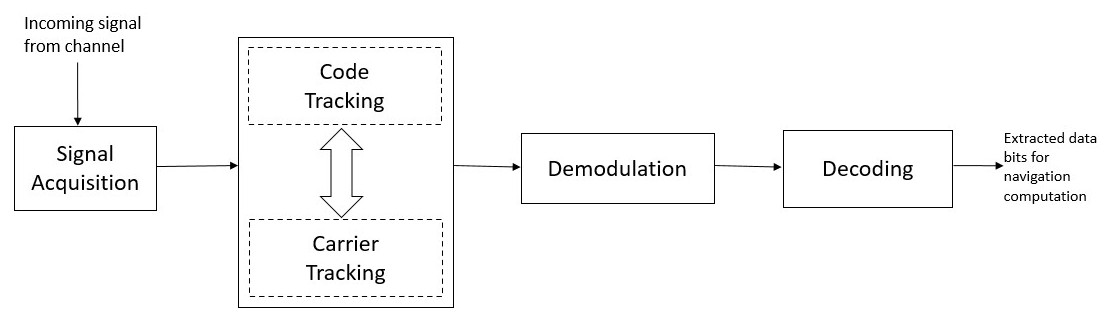
\includegraphics[width=1\columnwidth]{figs/signal_aq_tr.jpg}
		\centering
		\captionsetup{justification=centering}
		\caption{The Block Level Architecture for Receiver}
		\label{fig:demod_flow}
	\end{figure}
\end{normalsize}
\\
\\
\begin{enumerate}
	\item \textbf{Signal acquisition:} The receiver searches for and acquires the NavIC signal for a given satellite(s) by correlating the received signal with a locally generated replica of the spreading code used by the satellite(s). This process helps in identifying the presence of the NavIC signal and estimating coarse value of both doppler frequency shift and code delay.
\item \textbf{Carrier tracking:} Once the signal is acquired, the receiver performs carrier tracking to estimate and track the carrier frequency and phase of the received signal. This is crucial for demodulation as it ensures accurate demodulation of the navigation message and ranging signal.
\item \textbf{Code delay tracking:} The receiver performs code delay tracking to estimate and track the spreading code used by the satellites. This helps in maintaining synchronization with the transmitted signal and extracting the navigation data and ranging information.
\item \textbf{Signal demodulation:}After the aquisition and tracking has been performed, the received data is mapped back using BPSK demodulation, mapping $-1$ to binary $1$ and $+1$ to binary $0$.
\item \textbf{Signal decoding:} Once the signal has been demodulated, the decoding is performed removing all the extra bits that were added to navigation data during the encoding process.
\end{enumerate}

\section{Signal Acquistion}
The role of the aqusition block is to examine the presence/absence of signals coming from a given satellite. In the case of signal being present, it should provide coarse estimations of the Code delay and the Carrier Doppler shift, yet accurate enough to initialize the frequency and code tracking loops.
\\
\\
A generic IRNSS signal defined by its complex baseband equivalent, 
$S_T(t)$, the digital signal at the input of an Acquisition block can be written as:
\begin{align}
	x_{IN}[k]=A(t)\hat s_T (t-\tau(t))e^{j(2 \pi f_D(t)t+\Phi(t))}\bigg|_{t=kT_s} +n(t)\bigg|_{t=kT_s}
\end{align}
\begin{table}[h]
%\centering
%%%%%%%%%%%%%%%%%%%%%%%%%%%%%%%%%%%%%%%%%%%%%%%%%%%%%%%%%%%%%%%%%%%%%%
%%                                                                  %%
%%  This is the header of a LaTeX2e file exported from Gnumeric.    %%
%%                                                                  %%
%%  This file can be compiled as it stands or included in another   %%
%%  LaTeX document. The table is based on the longtable package so  %%
%%  the longtable options (headers, footers...) can be set in the   %%
%%  preamble section below (see PRAMBLE).                           %%
%%                                                                  %%
%%  To include the file in another, the following two lines must be %%
%%  in the including file:                                          %%
%%        \def\inputGnumericTable{}                                 %%
%%  at the beginning of the file and:                               %%
%%        \input{name-of-this-file.tex}                             %%
%%  where the table is to be placed. Note also that the including   %%
%%  file must use the following packages for the table to be        %%
%%  rendered correctly:                                             %%
%%    \usepackage[latin1]{inputenc}                                 %%
%%    \usepackage{color}                                            %%
%%    \usepackage{array}                                            %%
%%    \usepackage{longtable}                                        %%
%%    \usepackage{calc}                                             %%
%%    \usepackage{multirow}                                         %%
%%    \usepackage{hhline}                                           %%
%%    \usepackage{ifthen}                                           %%
%%  optionally (for landscape tables embedded in another document): %%
%%    \usepackage{lscape}                                           %%
%%                                                                  %%
%%%%%%%%%%%%%%%%%%%%%%%%%%%%%%%%%%%%%%%%%%%%%%%%%%%%%%%%%%%%%%%%%%%%%%



%%  This section checks if we are begin input into another file or  %%
%%  the file will be compiled alone. First use a macro taken from   %%
%%  the TeXbook ex 7.7 (suggestion of Han-Wen Nienhuys).            %%
\def\ifundefined#1{\expandafter\ifx\csname#1\endcsname\relax}


%%  Check for the \def token for inputed files. If it is not        %%
%%  defined, the file will be processed as a standalone and the     %%
%%  preamble will be used.                                          %%
\ifundefined{inputGnumericTable}

%%  We must be able to close or not the document at the end.        %%
	\def\gnumericTableEnd{\end{document}}


%%%%%%%%%%%%%%%%%%%%%%%%%%%%%%%%%%%%%%%%%%%%%%%%%%%%%%%%%%%%%%%%%%%%%%
%%                                                                  %%
%%  This is the PREAMBLE. Change these values to get the right      %%
%%  paper size and other niceties.                                  %%
%%                                                                  %%
%%%%%%%%%%%%%%%%%%%%%%%%%%%%%%%%%%%%%%%%%%%%%%%%%%%%%%%%%%%%%%%%%%%%%%

	\documentclass[12pt%
			  %,landscape%
                    ]{report}
       \usepackage[latin1]{inputenc}
       \usepackage{fullpage}
       \usepackage{color}
       \usepackage{array}
       \usepackage{longtable}
       \usepackage{calc}
       \usepackage{multirow}
       \usepackage{hhline}
       \usepackage{ifthen}

	\begin{document}


%%  End of the preamble for the standalone. The next section is for %%
%%  documents which are included into other LaTeX2e files.          %%
\else

%%  We are not a stand alone document. For a regular table, we will %%
%%  have no preamble and only define the closing to mean nothing.   %%
    \def\gnumericTableEnd{}

%%  If we want landscape mode in an embedded document, comment out  %%
%%  the line above and uncomment the two below. The table will      %%
%%  begin on a new page and run in landscape mode.                  %%
%       \def\gnumericTableEnd{\end{landscape}}
%       \begin{landscape}


%%  End of the else clause for this file being \input.              %%
\fi

%%%%%%%%%%%%%%%%%%%%%%%%%%%%%%%%%%%%%%%%%%%%%%%%%%%%%%%%%%%%%%%%%%%%%%
%%                                                                  %%
%%  The rest is the gnumeric table, except for the closing          %%
%%  statement. Changes below will alter the table's appearance.     %%
%%                                                                  %%
%%%%%%%%%%%%%%%%%%%%%%%%%%%%%%%%%%%%%%%%%%%%%%%%%%%%%%%%%%%%%%%%%%%%%%

\providecommand{\gnumericmathit}[1]{#1} 
%%  Uncomment the next line if you would like your numbers to be in %%
%%  italics if they are italizised in the gnumeric table.           %%
%\renewcommand{\gnumericmathit}[1]{\mathit{#1}}
\providecommand{\gnumericPB}[1]%
{\let\gnumericTemp=\\#1\let\\=\gnumericTemp\hspace{0pt}}
 \ifundefined{gnumericTableWidthDefined}
        \newlength{\gnumericTableWidth}
        \newlength{\gnumericTableWidthComplete}
        \newlength{\gnumericMultiRowLength}
        \global\def\gnumericTableWidthDefined{}
 \fi
%% The following setting protects this code from babel shorthands.  %%
 \ifthenelse{\isundefined{\languageshorthands}}{}{\languageshorthands{english}}
%%  The default table format retains the relative column widths of  %%
%%  gnumeric. They can easily be changed to c, r or l. In that case %%
%%  you may want to comment out the next line and uncomment the one %%
%%  thereafter                                                      %%
\providecommand\gnumbox{\makebox[0pt]}
%%\providecommand\gnumbox[1][]{\makebox}

%% to adjust positions in multirow situations                       %%
\setlength{\bigstrutjot}{\jot}
\setlength{\extrarowheight}{\doublerulesep}

%%  The \setlongtables command keeps column widths the same across  %%
%%  pages. Simply comment out next line for varying column widths.  %%
\setlongtables

\setlength\gnumericTableWidth{%
	68pt+%
	235pt+%
0pt}
\def\gumericNumCols{2}
\setlength\gnumericTableWidthComplete{\gnumericTableWidth+%
         \tabcolsep*\gumericNumCols*2+\arrayrulewidth*\gumericNumCols}
\ifthenelse{\lengthtest{\gnumericTableWidthComplete > \linewidth}}%
         {\def\gnumericScale{\ratio{\linewidth-%
                        \tabcolsep*\gumericNumCols*2-%
                        \arrayrulewidth*\gumericNumCols}%
{\gnumericTableWidth}}}%
{\def\gnumericScale{1}}

%%%%%%%%%%%%%%%%%%%%%%%%%%%%%%%%%%%%%%%%%%%%%%%%%%%%%%%%%%%%%%%%%%%%%%
%%                                                                  %%
%% The following are the widths of the various columns. We are      %%
%% defining them here because then they are easier to change.       %%
%% Depending on the cell formats we may use them more than once.    %%
%%                                                                  %%
%%%%%%%%%%%%%%%%%%%%%%%%%%%%%%%%%%%%%%%%%%%%%%%%%%%%%%%%%%%%%%%%%%%%%%

\ifthenelse{\isundefined{\gnumericColA}}{\newlength{\gnumericColA}}{}\settowidth{\gnumericColA}{\begin{tabular}{@{}p{68pt*\gnumericScale}@{}}x\end{tabular}}
\ifthenelse{\isundefined{\gnumericColB}}{\newlength{\gnumericColB}}{}\settowidth{\gnumericColB}{\begin{tabular}{@{}p{235pt*\gnumericScale}@{}}x\end{tabular}}

\begin{longtable}[c]{%
	b{\gnumericColA}%
	b{\gnumericColB}%
	}

%%%%%%%%%%%%%%%%%%%%%%%%%%%%%%%%%%%%%%%%%%%%%%%%%%%%%%%%%%%%%%%%%%%%%%
%%  The longtable options. (Caption, headers... see Goosens, p.124) %%
%	\caption{The Table Caption.}             \\	%
% \hline	% Across the top of the table.
%%  The rest of these options are table rows which are placed on    %%
%%  the first, last or every page. Use \multicolumn if you want.    %%

%%  Header for the first page.                                      %%
%	\multicolumn{2}{c}{The First Header} \\ \hline 
%	\multicolumn{1}{c}{colTag}	%Column 1
%	&\multicolumn{1}{c}{colTag}	\\ \hline %Last column
%	\endfirsthead

%%  The running header definition.                                  %%
%	\hline
%	\multicolumn{2}{l}{\ldots\small\slshape continued} \\ \hline
%	\multicolumn{1}{c}{colTag}	%Column 1
%	&\multicolumn{1}{c}{colTag}	\\ \hline %Last column
%	\endhead

%%  The running footer definition.                                  %%
%	\hline
%	\multicolumn{2}{r}{\small\slshape continued\ldots} \\
%	\endfoot

%%  The ending footer definition.                                   %%
%	\multicolumn{2}{c}{That's all folks} \\ \hline 
%	\endlastfoot
%%%%%%%%%%%%%%%%%%%%%%%%%%%%%%%%%%%%%%%%%%%%%%%%%%%%%%%%%%%%%%%%%%%%%%

\hhline{|-|-}
	 \multicolumn{1}{|p{\gnumericColA}|}%
	{\gnumericPB{\raggedright}\gnumbox[l]{\hspace{0.75cm}\textbf{Symbol}}}
	&\multicolumn{1}{p{\gnumericColB}|}%
	{\gnumericPB{\raggedright}\gnumbox[l]{\hspace{3cm} \textbf{Definition}}}
\\
\hhline{|--|}
	 \multicolumn{1}{|p{\gnumericColA}|}%
	{\gnumericPB{\raggedright}\gnumbox[l]{\hspace{1cm}$x_{IN}[k]$}}
	&\multicolumn{1}{p{\gnumericColB}|}%
	{\gnumericPB{\raggedright}\gnumbox[l]{Complex vector $I,Q$ samples of received signal}}
\\
\hhline{|--|}
	 \multicolumn{1}{|p{\gnumericColA}|}%
	{\gnumericPB{\raggedright}\gnumbox[l]{\hspace{1cm}A(t)}}
	&\multicolumn{1}{p{\gnumericColB}|}%
	{\gnumericPB{\raggedright}\gnumbox[l]{Signal Amplitude}}
\\
\hhline{|--|}
	 \multicolumn{1}{|p{\gnumericColA}|}%
	{\gnumericPB{\raggedright}\gnumbox[l]{\hspace{1cm}$\hat s_T(t)$}}
	&\multicolumn{1}{p{\gnumericColB}|}%
	{\gnumericPB{\raggedright}\gnumbox[l]{filtered version of $s_T(t)$}}
\\
\hhline{|--|}
	 \multicolumn{1}{|p{\gnumericColA}|}%
	{\gnumericPB{\raggedright}\gnumbox[l]{\hspace{1cm}$f_D(t)$ }}
	&\multicolumn{1}{p{\gnumericColB}|}%
	{\gnumericPB{\raggedright}\gnumbox[l]{Time varying doppler shift}}
\\
\hhline{|--|}
	 \multicolumn{1}{|p{\gnumericColA}|}%
	{\gnumericPB{\raggedright}\gnumbox[l]{\hspace{1cm}$\Phi (t)$}}
	&\multicolumn{1}{p{\gnumericColB}|}%
	{\gnumericPB{\raggedright}\gnumbox[l]{Time varying carrier phase shift}}
\\
\hhline{|--|}
	 \multicolumn{1}{|p{\gnumericColA}|}%
	{\gnumericPB{\raggedright}\gnumbox[l]{\hspace{1cm}$\tau (t)$}}
	&\multicolumn{1}{p{\gnumericColB}|}%
	{\gnumericPB{\raggedright}\gnumbox[l]{Time varying code delay}}
\\
\hhline{|--|}
	 \multicolumn{1}{|p{\gnumericColA}|}%
	{\gnumericPB{\raggedright}\gnumbox[l]{\hspace{1cm}n(t) }}
	&\multicolumn{1}{p{\gnumericColB}|}%
	{\gnumericPB{\raggedright}\gnumbox[l]{Time varying random noise}}
\\
\hhline{|--|}
	 \multicolumn{1}{|p{\gnumericColA}|}%
	{\gnumericPB{\raggedright}\gnumbox[l]{\hspace{1cm}$T_s$ }}
	&\multicolumn{1}{p{\gnumericColB}|}%
	{\gnumericPB{\raggedright}\gnumbox[l]{Sampling period}}
\\
\hhline{|-|-|}
\end{longtable}

\ifthenelse{\isundefined{\languageshorthands}}{}{\languageshorthands{\languagename}}
\gnumericTableEnd

\vspace{3mm}
\caption{Parameters Table in Signal Acquisition}
\label{table:table_para}
\end{table}

\subsection{Implementation of CA PCPS Acquisition}
The Parallel Code Phase Search (PCPS) algorithm is used in Acquisition block and is depicted in figure \ref{fig:pcps_flow} and described as follows:
\begin{normalsize}
\begin{figure}[ht]
	\centering
	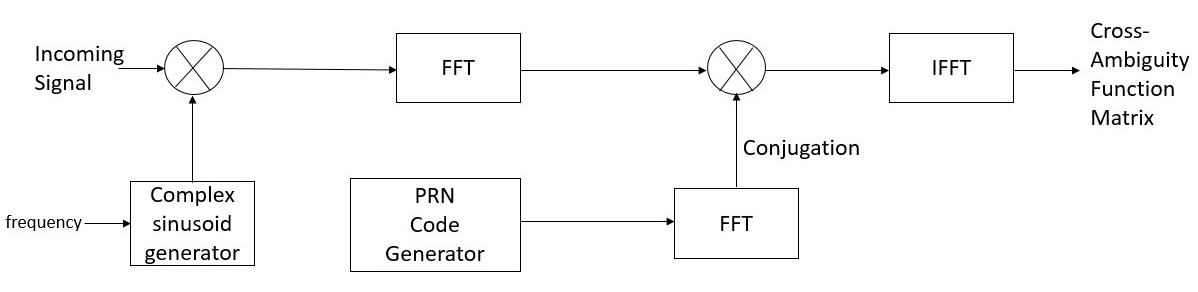
\includegraphics[width=1\columnwidth]{figs/pcps.jpg}
	\centering
	\captionsetup{justification=centering}
	\caption{PCPS algorithm flow}
	\label{fig:pcps_flow}
\end{figure}
\end{normalsize}
\\
\textbf{Given:}
\begin{enumerate}
	\item Input signal buffer $x_{IN}$ of K complex samples, provided by the Signal Conditioner 
	\item On-memory FFT of the local replica
	\begin{align}
		D[k]=FFT_K\{d[k]\}
	\end{align}
	\item Acquisition threshold  $\gamma$
	\item Frequency span : \sbrak{f_{min}, f_{max}}
	\item Frequency step : $f_{step}$
\end{enumerate}
\textbf{Expected:}
\begin{enumerate}
	\item Find out if signal is acquired or not for a given satellite(s) 
	\item If signal is acquired, for each given satellite, calculate coarse estimation of Doppler shift $\hat f_{D_{acq}}$ and Code delay $\hat \tau_{acq}$
\end{enumerate}
\textbf{Algorithm:}
\begin{enumerate}
	\item Calculate input signal power estimation  $\hat P_{in} = \frac{1}{K}\sum_{k=0}^{K-1} \big| x_{IN}[k]\big| ^2$
	\item for $\check f_D=[ f_{min} to f_{max}]\text{ in }f_{steps}$ 
	\begin{enumerate}
		\item Calculate carrier wipe off$\hspace{0.5cm}x[k]=x_{IN}[k]e^{-(j2 \pi \check f_D k T_s)}$,for $k=0,...,K-1$
		\item Calculate $X[k]=FFT_K\{x[k]\}$
		\item Calculate $Y[k]=X[k].D[k]$, for $k=0,...K-1$ 
        	\item Calculate corresponding column in the Cross ambiguity function matrix - $R_{xd}(\check f_D,\tau) = \frac{1}{K^2}IFFT_K\{Y[k]\}$
        \end{enumerate}

        \item Search maximum and its indices in the search grid:
	\begin{align}
		\{S_{max},f_i,\tau_j\} = max_{f,\tau} \big |R_{xd}(f,\tau)\big | ^2
	\end{align}
        \item	Calculate the Generalized Likelihood Ratio Test (GLRT) function with normalized variance:
	\begin{align}
		\Gamma_{GLRT} = \frac{2KS_{max}}{\hat P_{in}}
	\end{align}
	\item if $\Gamma_{GLRT} > \gamma$\\
	Declare positive acquisition and provides coarse estimation of code delay $\hat \tau_{acq} = \tau_j $ and Doppler shift $\hat f_{D_{acq}}=f_i$,\\
	other wise declare negative acquisition.\\
\end{enumerate}
The acquisition results are generated using the below code\\
\textbf{Code}
\begin{lstlisting}
	code/e2e_sim/main.ipynb
\end{lstlisting}

\section{Tracking}
The role of tracking block is to follow signal synchronization parameters: code phase, Doppler shift and carrier phase and extract the baseband signal. It performs the following 3 function to decipher the baseband signal from the incoming signal as shown in figure \ref{fig:tracking}. 
\begin{enumerate}
	\item Carrier and code wipeoff 
	\item Pre-detection integration
	\item Baseband signal processing
\end{enumerate}

\begin{normalsize}
\begin{figure}[ht]
\centering
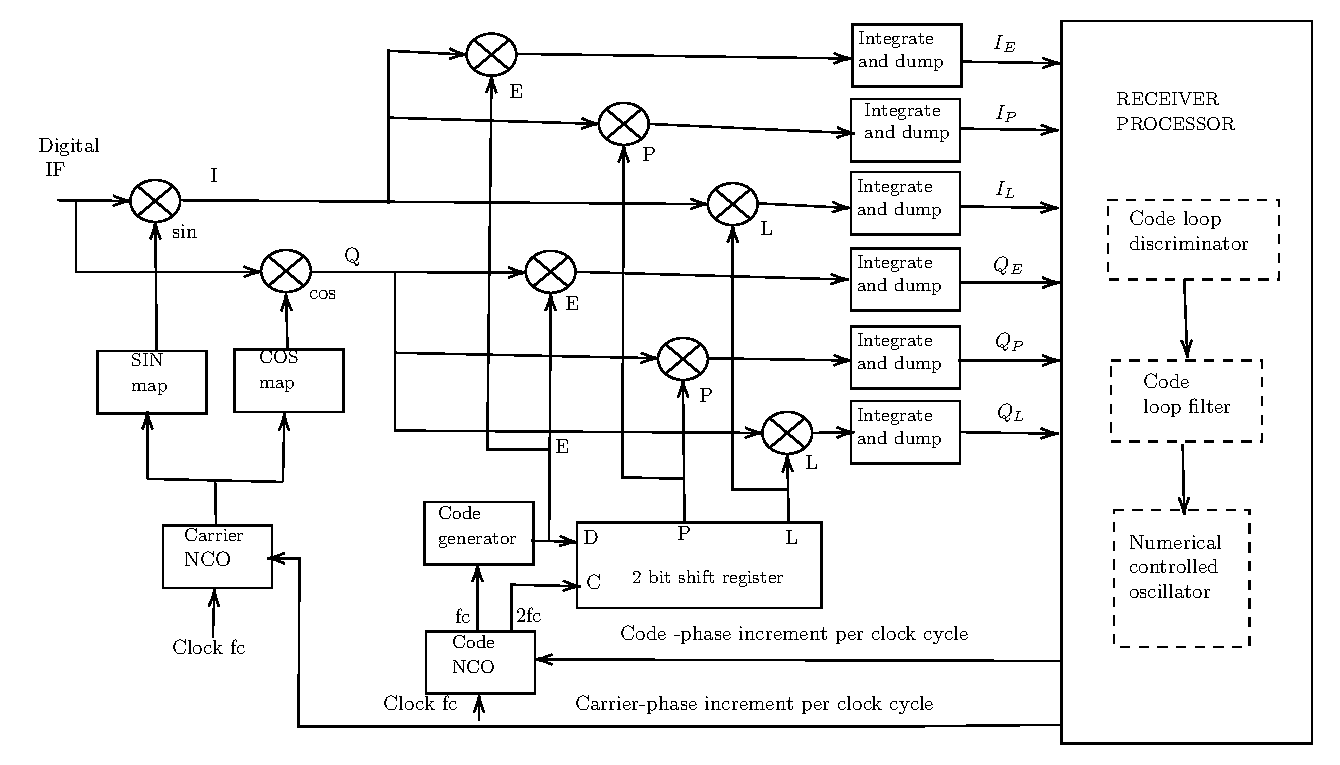
\includegraphics[width=1\columnwidth]{figs/block3}
\centering
\captionsetup{justification=centering}
\caption{Tracking block diagram}
\label{fig:tracking}
\end{figure}
\end{normalsize}
\subsection{Carrier and code wipeoff}
\textbf{Carrier wipeoff: }Referring to the figure \ref{fig:tracking}, first the digital IF is stripped off the carrier (plus carrier Doppler) by the replica carrier (plus carrier Doppler) signals to produce in-phase (I) and quadraphase (Q) sampled data. The I and Q signals at the outputs of the mixers have the desired phase relationships with respect to the detected carrier of the desired satellite. The replica carrier (including carrier Doppler) signals are synthesized by the carrier numerically controlled oscillator (NCO) and the discrete sine and cosine mapping functions. In closed loop operation, the carrier NCO is controlled by the carrier tracking loop in the receiver processor.
\\
\textbf{Code wipeoff: } The I and Q signals are then correlated with early(E), prompt(P), and late(L) replica codes (plus code Doppler) synthesized by the code generator, a 2-bit shift register, and the code NCO. In closed loop operation, the code NCO is controlled by the code tracking loop in the receiver processor. E and L are typically separated in phase by 1 chip and P is in the middle. The prompt replica code phase is aligned with the incoming satellite code phase producing maximum correlation if it is tracking the incoming satellite code phase. Under this circumstance, the early phase is aligned a fraction of a chip period early, and the late phase is aligned the same fraction of the chip period late with respect to the incoming  code phase, and these correlators produce about half the maximum correlation. Any misalignment in the replica code phase with respect to the incoming code phase produces a difference in the vector magnitudes of the early and late correlated outputs so that the amount and direction of the phase change can be detected and corrected by the code tracking loop.
\subsection{Pre-detection and integration}
Extensive digital predetection integration and dump processes occur after the carrier and code wiping off processes. Figure \ref{fig:tracking} shows three complex correlators required to produce three in-phase
components, which are integrated and dumped to produce $I_E , I_P , I_L$ and three quadraphase components integrated and dumped to produce $Q_E , Q_P , Q_L$ . The carrier wipeoff and code wipeoff processes must be performed at the digital IF sample rate, while the integrate and dump accumulators provide filtering and resampling at the processor baseband input rate, which can be at 1,000 Hz during search modes or as low as 50 Hz during
track modes, depending on the desired dwell time during search or the desired predetection integration time during track.
\subsection{Baseband signal processing}
This entails Carrier tracking and Code tracking using Phase locked loop (PLL), Frequency locked loop (FLL) and Delay locked loop (DLL). The general block diagram is as shown in Figure \ref{fig:Carrier_Code_Tracking}. 

\begin{normalsize}
	\begin{figure}[ht]
		\centering
		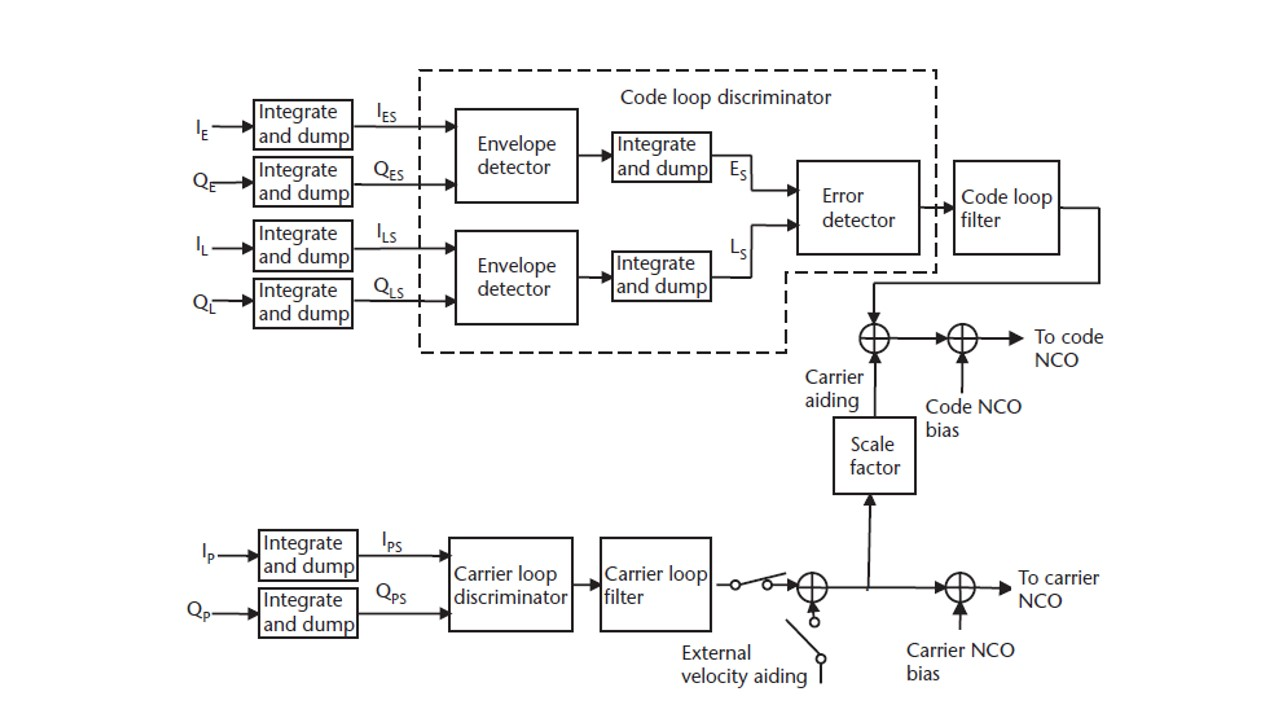
\includegraphics[width=1\columnwidth]{figs/tracking_loop}
		\centering
		\captionsetup{justification=centering}
		\caption{Generic baseband processor code and carrier tracking loops block diagram}
		\label{fig:Carrier_Code_Tracking}
	\end{figure}
\end{normalsize}

\subsubsection{Carrier tracking loop}
\textbf{Phase locked loop(PLL)}\\
The carrier loop discriminator defines the type of tracking loop as a PLL, a Costas PLL (which is a PLL-type discriminator that tolerates the presence of data modulation on the baseband signal), or a frequency lock loop (FLL). Carrier tracking loop tracks the frequency and phase of the received signal by detecting the phase error between replicated signal and incoming signal and accordingly replicated signal produced by numerically controlled oscillator (NCO) is adjusted to synchronize with incoming signal in both frequency and phase. For zero phase error detected, navigation data is accurately extracted. 
\begin{align}
  \text{Phase error} =ATAN2(I_P,Q_P) = \tan^{-1}\brak{\frac{I_P}{Q_P}}
\end{align}
The ATAN2 discriminator is the only one that remains linear over the full input error range of $\pm180^{\circ}$. However, in the presence of noise, both of the discriminator outputs are linear only near the $0^{\circ}$ region. These PLL discriminators will achieve the 6-dB improvement in signal tracking threshold (by comparison with the Costas discriminators) for the dataless carrier because they track the full four quadrant range of the input signal.
\\
\\
\textbf{Frequency locked loop}\\
PLLs replicate the exact phase and frequency of the incoming SV (converted to IF) to perform the carrier wipeoff function. FLLs perform the carrier wipeoff process by replicating the approximate frequency, and they typically permit the phase to rotate with respect to the incoming carrier signal. The algorithm used in FLL discriminator is $\frac{\text{ATAN2}{\brak{cross,dot}}}{t_2-t_1}$. The frequency error is given by 
\begin{align}
	\text{Frequency error} = \frac{\phi_2-\phi_1}{t_2-t_1}
\end{align}

\noindent The pahse change $\phi_2 - \phi_1$ between two adjacent samples of $I_{PS}$ and $Q_{PS}$ at times $t_2$ and $t_1$ is computed. This phase change in a fixed interval of time is proportinal to frequenct error in the carrier tracking loop. The error is fed to carier NCO to adjust the frequency to lock to the right frequency.

\subsubsection{Code tracking loop}
\textbf{Delay locked loop:}
Post the carrier signal synchronization, received CA code samples are synchronized by aligning with replicated CA code samples by shifting right or left. To determine the direction of shift, the I and Q outputs are multiplied with prompt code (PRN code which is phase aligned), early code (prompt PRN code shifted by some samples to the right) and late code (prompt PRN code shifted by some samples to the left) resulting in corresponding to I and Q channel respectively. Following algorithm is used to lock the code phase.

\begin{align}
	E&=\sqrt[]{I_{ES}^2+Q_{ES}^2}\\
	L&=\sqrt[]{I_{LS}^2+Q_{LS}^2}
\end{align}

\begin{align}
	\text{DLL Discriminator} (\epsilon)&=\frac{1}{2}\frac{E-L}{E+L}
\end{align}

\noindent If the replica code is aligned, then the early and late envelopes are equal in amplitude and no error is generated by the discriminator. If the replica code is misaligned, then the early and late envelopes are unequal by an amount that is proportional to the amount of code phase error between the replica and the incoming signal (within the limits of the correlation interval). The code discriminator senses the amount of error in the replica code and the direction (early or late) from the difference in the amplitudes of the early and late envelopes. This
error is filtered and then applied to the code loop NCO, where the output code shift is increased or decreased as necessary to correct the replica code generator phase with respect to the incoming SV signal code phase.

\subsubsection{Loop filter characteristics}
\begin{table}[h]
%\centering
%%%%%%%%%%%%%%%%%%%%%%%%%%%%%%%%%%%%%%%%%%%%%%%%%%%%%%%%%%%%%%%%%%%%%%
%%                                                                  %%
%%  This is the header of a LaTeX2e file exported from Gnumeric.    %%
%%                                                                  %%
%%  This file can be compiled as it stands or included in another   %%
%%  LaTeX document. The table is based on the longtable package so  %%
%%  the longtable options (headers, footers...) can be set in the   %%
%%  preamble section below (see PRAMBLE).                           %%
%%                                                                  %%
%%  To include the file in another, the following two lines must be %%
%%  in the including file:                                          %%
%%        \def\inputGnumericTable{}                                 %%
%%  at the beginning of the file and:                               %%
%%        \input{name-of-this-file.tex}                             %%
%%  where the table is to be placed. Note also that the including   %%
%%  file must use the following packages for the table to be        %%
%%  rendered correctly:                                             %%
%%    \usepackage[latin1]{inputenc}                                 %%
%%    \usepackage{color}                                            %%
%%    \usepackage{array}                                            %%
%%    \usepackage{longtable}                                        %%
%%    \usepackage{calc}                                             %%
%%    \usepackage{multirow}                                         %%
%%    \usepackage{hhline}                                           %%
%%    \usepackage{ifthen}                                           %%
%%  optionally (for landscape tables embedded in another document): %%
%%    \usepackage{lscape}                                           %%
%%                                                                  %%
%%%%%%%%%%%%%%%%%%%%%%%%%%%%%%%%%%%%%%%%%%%%%%%%%%%%%%%%%%%%%%%%%%%%%%



%%  This section checks if we are begin input into another file or  %%
%%  the file will be compiled alone. First use a macro taken from   %%
%%  the TeXbook ex 7.7 (suggestion of Han-Wen Nienhuys).            %%
\def\ifundefined#1{\expandafter\ifx\csname#1\endcsname\relax}


%%  Check for the \def token for inputed files. If it is not        %%
%%  defined, the file will be processed as a standalone and the     %%
%%  preamble will be used.                                          %%
\ifundefined{inputGnumericTable}

%%  We must be able to close or not the document at the end.        %%
	\def\gnumericTableEnd{\end{document}}


%%%%%%%%%%%%%%%%%%%%%%%%%%%%%%%%%%%%%%%%%%%%%%%%%%%%%%%%%%%%%%%%%%%%%%
%%                                                                  %%
%%  This is the PREAMBLE. Change these values to get the right      %%
%%  paper size and other niceties.                                  %%
%%                                                                  %%
%%%%%%%%%%%%%%%%%%%%%%%%%%%%%%%%%%%%%%%%%%%%%%%%%%%%%%%%%%%%%%%%%%%%%%

	\documentclass[12pt%
			  %,landscape%
                    ]{report}
       \usepackage[latin1]{inputenc}
       \usepackage{fullpage}
       \usepackage{color}
       \usepackage{array}
       \usepackage{longtable}
       \usepackage{calc}
       \usepackage{multirow}
       \usepackage{hhline}
       \usepackage{ifthen}

	\begin{document}


%%  End of the preamble for the standalone. The next section is for %%
%%  documents which are included into other LaTeX2e files.          %%
\else

%%  We are not a stand alone document. For a regular table, we will %%
%%  have no preamble and only define the closing to mean nothing.   %%
    \def\gnumericTableEnd{}

%%  If we want landscape mode in an embedded document, comment out  %%
%%  the line above and uncomment the two below. The table will      %%
%%  begin on a new page and run in landscape mode.                  %%
%       \def\gnumericTableEnd{\end{landscape}}
%       \begin{landscape}


%%  End of the else clause for this file being \input.              %%
\fi

%%%%%%%%%%%%%%%%%%%%%%%%%%%%%%%%%%%%%%%%%%%%%%%%%%%%%%%%%%%%%%%%%%%%%%
%%                                                                  %%
%%  The rest is the gnumeric table, except for the closing          %%
%%  statement. Changes below will alter the table's appearance.     %%
%%                                                                  %%
%%%%%%%%%%%%%%%%%%%%%%%%%%%%%%%%%%%%%%%%%%%%%%%%%%%%%%%%%%%%%%%%%%%%%%

\providecommand{\gnumericmathit}[1]{#1} 
%%  Uncomment the next line if you would like your numbers to be in %%
%%  italics if they are italizised in the gnumeric table.           %%
%\renewcommand{\gnumericmathit}[1]{\mathit{#1}}
\providecommand{\gnumericPB}[1]%
{\let\gnumericTemp=\\#1\let\\=\gnumericTemp\hspace{0pt}}
 \ifundefined{gnumericTableWidthDefined}
        \newlength{\gnumericTableWidth}
        \newlength{\gnumericTableWidthComplete}
        \newlength{\gnumericMultiRowLength}
        \global\def\gnumericTableWidthDefined{}
 \fi
%% The following setting protects this code from babel shorthands.  %%
 \ifthenelse{\isundefined{\languageshorthands}}{}{\languageshorthands{english}}
%%  The default table format retains the relative column widths of  %%
%%  gnumeric. They can easily be changed to c, r or l. In that case %%
%%  you may want to comment out the next line and uncomment the one %%
%%  thereafter                                                      %%
\providecommand\gnumbox{\makebox[0pt]}
%%\providecommand\gnumbox[1][]{\makebox}

%% to adjust positions in multirow situations                       %%
\setlength{\bigstrutjot}{\jot}
\setlength{\extrarowheight}{\doublerulesep}

%%  The \setlongtables command keeps column widths the same across  %%
%%  pages. Simply comment out next line for varying column widths.  %%
\setlongtables

\setlength\gnumericTableWidth{%
	70pt+%
	100pt+%
	80pt+%
0pt}
\def\gumericNumCols{3}
\setlength\gnumericTableWidthComplete{\gnumericTableWidth+%
         \tabcolsep*\gumericNumCols*2+\arrayrulewidth*\gumericNumCols}
\ifthenelse{\lengthtest{\gnumericTableWidthComplete > \linewidth}}%
         {\def\gnumericScale{\ratio{\linewidth-%
                        \tabcolsep*\gumericNumCols*2-%
                        \arrayrulewidth*\gumericNumCols}%
{\gnumericTableWidth}}}%
{\def\gnumericScale{1}}

%%%%%%%%%%%%%%%%%%%%%%%%%%%%%%%%%%%%%%%%%%%%%%%%%%%%%%%%%%%%%%%%%%%%%%
%%                                                                  %%
%% The following are the widths of the various columns. We are      %%
%% defining them here because then they are easier to change.       %%
%% Depending on the cell formats we may use them more than once.    %%
%%                                                                  %%
%%%%%%%%%%%%%%%%%%%%%%%%%%%%%%%%%%%%%%%%%%%%%%%%%%%%%%%%%%%%%%%%%%%%%%

\ifthenelse{\isundefined{\gnumericColA}}{\newlength{\gnumericColA}}{}\settowidth{\gnumericColA}{\begin{tabular}{@{}p{70pt*\gnumericScale}@{}}x\end{tabular}}
\ifthenelse{\isundefined{\gnumericColB}}{\newlength{\gnumericColB}}{}\settowidth{\gnumericColB}{\begin{tabular}{@{}p{100pt*\gnumericScale}@{}}x\end{tabular}}
\ifthenelse{\isundefined{\gnumericColC}}{\newlength{\gnumericColC}}{}\settowidth{\gnumericColC}{\begin{tabular}{@{}p{80pt*\gnumericScale}@{}}x\end{tabular}}

\begin{longtable}[c]{%
	b{\gnumericColA}%
	b{\gnumericColB}%
	b{\gnumericColC}%
	}

%%%%%%%%%%%%%%%%%%%%%%%%%%%%%%%%%%%%%%%%%%%%%%%%%%%%%%%%%%%%%%%%%%%%%%
%%  The longtable options. (Caption, headers... see Goosens, p.124) %%
%	\caption{The Table Caption.}             \\	%
% \hline	% Across the top of the table.
%%  The rest of these options are table rows which are placed on    %%
%%  the first, last or every page. Use \multicolumn if you want.    %%

%%  Header for the first page.                                      %%
%	\multicolumn{3}{c}{The First Header} \\ \hline 
%	\multicolumn{1}{c}{colTag}	%Column 1
%	&\multicolumn{1}{c}{colTag}	%Column 2
%	&\multicolumn{1}{c}{colTag}	\\ \hline %Last column
%	\endfirsthead

%%  The running header definition.                                  %%
%	\hline
%	\multicolumn{3}{l}{\ldots\small\slshape continued} \\ \hline
%	\multicolumn{1}{c}{colTag}	%Column 1
%	&\multicolumn{1}{c}{colTag}	%Column 2
%	&\multicolumn{1}{c}{colTag}	\\ \hline %Last column
%	\endhead

%%  The running footer definition.                                  %%
%	\hline
%	\multicolumn{3}{r}{\small\slshape continued\ldots} \\
%	\endfoot

%%  The ending footer definition.                                   %%
%	\multicolumn{3}{c}{That's all folks} \\ \hline 
%	\endlastfoot
%%%%%%%%%%%%%%%%%%%%%%%%%%%%%%%%%%%%%%%%%%%%%%%%%%%%%%%%%%%%%%%%%%%%%%

\hhline{|-|-|-}
	 \multicolumn{1}{|p{\gnumericColA}|}%
	{\gnumericPB{\raggedright}\gnumbox[l]{\textbf{Loop Order}}}
	&\multicolumn{1}{p{\gnumericColB}|}%
	{\gnumericPB{\raggedright}\gnumbox[l]{\textbf{Noise Bandwidth}}}
	&\multicolumn{1}{p{\gnumericColC}|}%
	{\gnumericPB{\raggedright}\gnumbox[l]{\textbf{Typical Filter  }}}
\\
%\hhline{|---|}
	 \multicolumn{1}{|p{\gnumericColA}|}%
	{\gnumericPB{\raggedleft}\gnumbox[r]{}}
	&\multicolumn{1}{p{\gnumericColB}|}%
	{\gnumericPB{\raggedright}\gnumbox[l]{\textbf{$ B_n$ (Hz)}}}
	&\multicolumn{1}{p{\gnumericColC}|}%
	{\gnumericPB{\raggedright}\gnumbox[l]{\textbf{ Values }}}
	%{\gnumericPB{\raggedright}\gnumbox[l]{}}\\
	\\
\hhline{|---|}
	 \multicolumn{1}{|p{\gnumericColA}|}%
	{\gnumericPB{\raggedleft}\gnumbox[r]{First}}
	&\multicolumn{1}{p{\gnumericColB}|}%
	{\gnumericPB{\raggedright}\gnumbox[l]{\hspace{0.5cm}$\frac{\omega_o}{4}$}}
	&\multicolumn{1}{p{\gnumericColC}|}%
	{\gnumericPB{\raggedright}\gnumbox[l]{\hspace{0.5cm}$\omega_o $ }}
	%{\gnumericPB{\raggedright}\gnumbox[l]{}}\\
	\\
%\hhline{|---|}
	 \multicolumn{1}{|p{\gnumericColA}|}%
	{\gnumericPB{\raggedleft}\gnumbox[r]{}}
	&\multicolumn{1}{p{\gnumericColB}|}%
	{\gnumericPB{\raggedright}\gnumbox[l]{}}
	&\multicolumn{1}{p{\gnumericColC}|}%
	{\gnumericPB{\raggedright}\gnumbox[l]{ $B_n=0.25\omega_o$}}
\\
\hhline{|---|}
\multicolumn{1}{|p{\gnumericColA}|}%
	{\gnumericPB{\raggedleft}\gnumbox[r]{}}
	&\multicolumn{1}{p{\gnumericColB}|}%
	{\gnumericPB{\raggedright}\gnumbox[l]{}}
	&\multicolumn{1}{p{\gnumericColC}|}%
	{\gnumericPB{\raggedright}\gnumbox[l]{ $\omega_o^2$}}
	 
\\
%\hhline{|---|}
	\multicolumn{1}{|p{\gnumericColA}|}%
	{\gnumericPB{\raggedleft}\gnumbox[r]{Second}}
	&\multicolumn{1}{p{\gnumericColB}|}%
	{\gnumericPB{\raggedright}\gnumbox[l]{$\frac{\omega(1+a_2^2)}{4a_2}$}}
	&\multicolumn{1}{p{\gnumericColC}|}%
	{\gnumericPB{\raggedright}\gnumbox[l]{$a_2\omega_o=1.414\omega_o$}}
\\
%\hhline{|-|-|-|}
\multicolumn{1}{|p{\gnumericColA}|}%
	{\gnumericPB{\raggedleft}\gnumbox[r]{}}
	&\multicolumn{1}{p{\gnumericColB}|}%
	{\gnumericPB{\raggedright}\gnumbox[l]{}}
	&\multicolumn{1}{p{\gnumericColC}|}%
	{\gnumericPB{\raggedright}\gnumbox[l]{ $B_n=0.53\omega_o$}}
	
	\\
\hhline{|-|-|-|}
 \multicolumn{1}{|p{\gnumericColA}|}%
	{\gnumericPB{\raggedleft}\gnumbox[r]{}}
	&\multicolumn{1}{p{\gnumericColB}|}%
	{\gnumericPB{\raggedright}\gnumbox[l]{}}
	&\multicolumn{1}{p{\gnumericColC}|}%
	{\gnumericPB{\raggedright}\gnumbox[l]{$\omega_o^3$ }}
		\\
%\hhline{|-|-|-|}
 \multicolumn{1}{|p{\gnumericColA}|}%
	{\gnumericPB{\raggedleft}\gnumbox[r]{Third}}
	&\multicolumn{1}{p{\gnumericColB}|}%
	{\gnumericPB{\raggedright}\gnumbox[l]{$\frac{\omega(a_3b_3^2+a_3^2-b_3)}{4(a_3b_3-1)}$}}
	&\multicolumn{1}{p{\gnumericColC}|}%
	{\gnumericPB{\raggedright}\gnumbox[l]{$ a_3\omega_o^2=1.1\omega_o^2$}}
	\\
%\hhline{|-|-|-|}
 \multicolumn{1}{|p{\gnumericColA}|}%
	{\gnumericPB{\raggedleft}\gnumbox[r]{}}
	&\multicolumn{1}{p{\gnumericColB}|}%
	{\gnumericPB{\raggedright}\gnumbox[l]{}}
	&\multicolumn{1}{p{\gnumericColC}|}%
	{\gnumericPB{\raggedright}\gnumbox[l]{$b_3\omega_o=2.4\omega_o$}}
	\\
%\hhline{|-|-|-|}
 \multicolumn{1}{|p{\gnumericColA}|}%
	{\gnumericPB{\raggedleft}\gnumbox[r]{}}
	&\multicolumn{1}{p{\gnumericColB}|}%
	{\gnumericPB{\raggedright}\gnumbox[l]{}}
	&\multicolumn{1}{p{\gnumericColC}|}%
	{\gnumericPB{\raggedright}\gnumbox[l]{ $B_n=0.7845\omega_o$}}
		\\
\hhline{|-|-|-|}
 
\end{longtable}

\ifthenelse{\isundefined{\languageshorthands}}{}{\languageshorthands{\languagename}}
\gnumericTableEnd

\vspace{3mm}
\caption{Loop order filters}
\label{table:loop}
\end{table}
\noindent The values for the second-order coefficient $a_2$ and third-order coefficients $a_3$ and $b_3$ can be determined from Table 3. These coefficients are the same for FLL, PLL, or DLL applications if the loop
order and the noise bandwidth,$B_n$ , are the same.Note that the FLL coefficient insertion point into the filter is one integrator back from the PLL and DLL insertion points.This is because the FLL error is in units of hertz (change in range per unit of time).

\section{Demodulation}
Demodulation is the process of extracting the original information or baseband signal from a modulated carrier signal. The purpose of demodulation is to retrieve the modulating signal, which could be analog or digital data, audio, video, or other forms of information. Demodulation is essential in various communication systems such as radio, television, cellular networks, and wireless data transmission.
\\
\\
After the aquisition and tracking has been performed, the received data is mapped back using BPSK demodulation, mapping $-1$ to binary $1$ and $+1$ to binary $0$.

\section{Synchronization and Decoding}
\subsection{Synchronization}
Synchronization involves bit and frame synchronization
\\\textbf{Bit Synchronization}: %The output of tracking block produces at a sample rate of 1000sps. Nav datarate is 50bps. To correctly decode the nav data, data from tracking block must be converted from 1000sps to 50bps. Therefore, we need to replace 20 consecutive values with 1 value.%
Post Tracking section, each code block with boundary of 1ms is known. This 1ms is integrated in tracking section to get 1 sample. Each databit consists 20 such samples corresponding to 20 ms. We flag the location where maximum number of transitions occured to get bit boundary in each block of 20ms.\\
\textbf{Frame Synchronizaton}:\\
Frame synchronization determines the exact start and endpoint of a subframe. Each subframe starts with  16 bit sync word. The sync pattern is EB90 Hex.\\
Demodulated data is deintrleaved and sent to Channel decoding module for further processing. The deinterleaving process involves reversing the interleaving algorithm used during transmission. By applying the inverse operation, the interleaved data are rearranged back into their original order. 
Channel decoding involves the process of error correction and retrieval of the original data transmitted over the satellite link. The channel decoding scheme used in NavIC is based on a convolutional coding technique known as Rate 1/2 Convolutional Code with Viterbi decoding.
\subsection{Decoding}
The high-level description of the channel decoding process in NavIC is shown in figure \ref{fig:decoding_r}
\begin{normalsize}
\begin{figure}[ht]
\centering
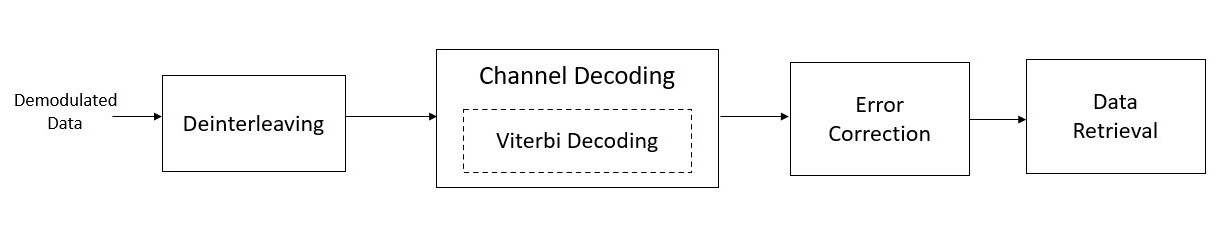
\includegraphics[width=1\columnwidth]{figs/decoding_r.jpg}
\centering
\captionsetup{justification=centering}
\caption{The Block Level Architecture for Channel decoding}
\label{fig:decoding_r}
\end{figure}
\end{normalsize}


\subsection{Convolutional Code Representation}

The convolutional code is represented as a state diagram or Trellis, where each state represents a unique history of the encoded bits.
The Trellis consists of nodes and branches. Nodes correspond to states, and branches represent transitions between states.
Each branch is labeled with the input bit and the encoded output bits associated with the transition.

\subsubsection{Branch Metrics}
At each time step, the Viterbi algorithm calculates branch metrics, which quantify the similarity between the received signal and the expected signal for each branch.
The branch metric is typically based on a distance measure, such as Hamming distance or Euclidean distance, between the received signal and the expected signal.
Let's denote the received signal at time step t as r(t) and the expected signal for a particular branch as c(t). The branch metric B(t) for that branch at time step t is computed as the distance between r(t) and c(t).

\subsubsection{Path Metrics}
The Viterbi algorithm computes a path metric for each state at each time step, which represents the accumulated likelihood of reaching that state along a particular path.
The path metric is typically computed as the minimum (or maximum, depending on the metric used) of the sum of the previous path metric and the branch metric.
Let's denote the path metric for state i at time step t as P(i, t). The path metric for state i at time step t is computed as:
\begin{center}
P(i, t) = min{P(j, t-1) + B(t)}, where j is the previous state connected to state i.
\end{center}

\subsubsection{Survivor Paths}
Along with the path metrics, the Viterbi algorithm keeps track of survivor paths, which represent the most likely paths leading to each state at each time step.
The survivor paths are determined based on the branch with the smallest (or largest, depending on the metric used) branch metric leading to each state.
The survivor paths help in traceback, as they indicate the most likely sequence of states leading to the current state.

\subsubsection{Traceback}
Once the decoding reaches the end of the received signal, a traceback process is performed to determine the final decoded sequence.
Starting from the state with the highest path metric at the last time step, the algorithm traces back through the trellis by following the survivor paths.
The traceback process continues until reaching the starting state at the first time step, yielding the decoded sequence of transmitted bits.

\subsection{Decoding Output}
The traceback process generates the final decoded output, which should ideally match the original transmitted data. Nav data contains tail bits, i.e., 6 zero value bits that enables completion of FEC decoding of each subframe in the user receiver.
To further enhance the reliability of the decoded sequence by correcting errors, advanced codes like Reed Solomon codes can be used.

\noindent The Viterbi algorithm is an iterative process that calculates and updates the path metrics and survivor paths at each time step. It efficiently explores all possible paths through the trellis and selects the most likely path. This results in the recovery of the transmitted data even in the presence of noise and errors.

\subsection{Example}
In the figure \ref{fig:Trellis},
\begin{normalsize}
\begin{figure}[ht]
	\centering
	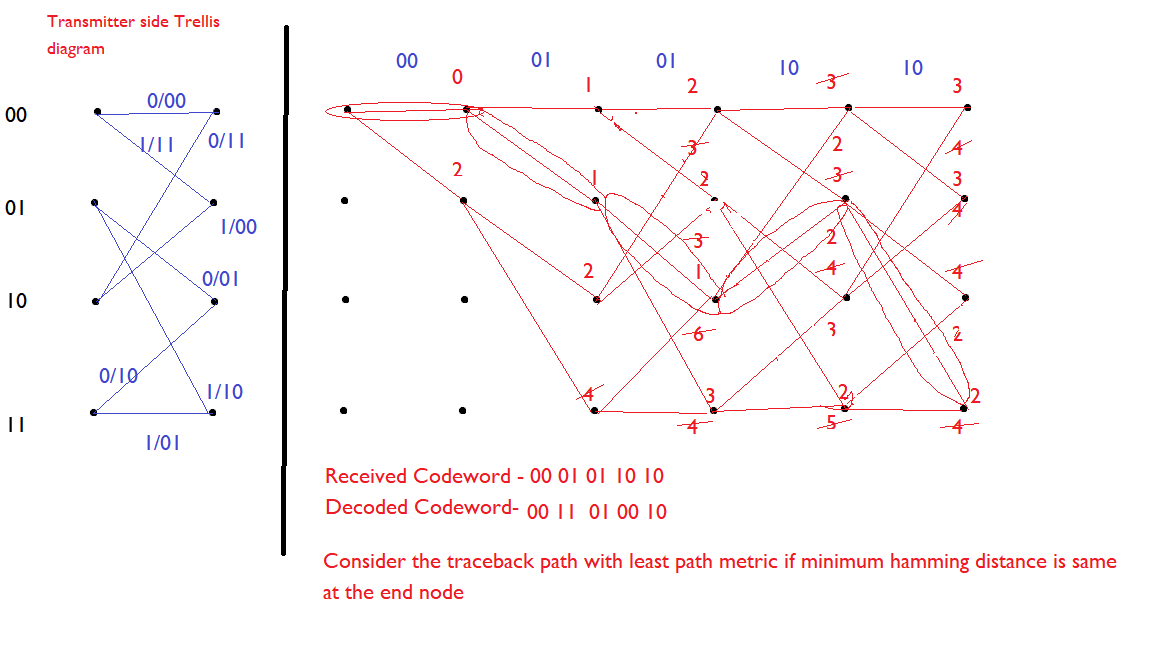
\includegraphics[width=1\columnwidth]{figs/Trellis_navic.png}
	\centering
	\captionsetup{justification=centering}
	\caption{Trellis flow for Viterbi algorithm}
	\label{fig:Trellis}
\end{figure}
\end{normalsize}


\textbf{Transmitter side:} 

\noindent Left most 00, 01, 10, 11 - are the state s0, s1, s2 and s3 at time t. a/bb means, for input a, output is bb for a given state transition.
\\
\textbf{Receiver side:} 

\noindent Assume the bits at top are received codewords - \textbf{00 01 01 10 10}. The codewords are compared with the possible transition states from the input diagram, thereby calculating hamming distance between received and possible outputs as per Trellis diagram. For example, for codeword $00$, state is $00$ and two possible paths are drawn in red. Hamming distance is calculated between received codeword $00$ and possible outputs - $00, 11$.

\noindent Similarly in the next step, for codeword $01$, possible paths are from state $00$ and state $01$. Hence, hamming distance is calculated for all possible paths. When a node has 2 or more inputs, the least hamming distance is chosen. Branch metric is the minimum hamming distance value for a given path. Path metric is the sum of previously calculated path metric and current branch metric. At the end, if the path metric value is equal for 2 different traceback paths, they are chosen with equal probability.

\noindent The process continues till the final codeword $10$ is examined. Finally, a path with the least values of path metric is chosen. In this case the path from end to start is marked in the figure \ref{fig:Trellis}. The decoded codeword is determined as \textbf{00 11 01 00 10}.
\\
\\
The functions for acquisition and tracking are present in the below code
\begin{lstlisting}
codes/demodulation/demodulation.py
\end{lstlisting}
The functions for decoding are present in the below code
\begin{center}
 \begin{lstlisting}
codes/decoder/decode.py
 \end{lstlisting}
\end{center}
The tracking results are generated using the code below and the plot is shown in figure \ref{fig:tracking_plot}.\\
\textbf{Code}
\begin{lstlisting}
code/e2e_sim/main_ipynb
\end{lstlisting}








\chapter{Real time Implementation of Transmiter and Receiver}
\section{Transmitter implementaion}

\subsection{Installations for Transmitter module}
\begin{lstlisting}
sudo apt update
sudo apt install build-essential
sudo apt install make
\end{lstlisting}

\subsection{Generating the real time samples using Tranmitter module}
\begin{enumerate}
    \item Clone the transmitter module from below
    \begin{lstlisting}
        gvv/navic_L5_POC/codes/navic_transmiter
    \end{lstlisting}
    \item Build the project 
    \begin{lstlisting}
        make
    \end{lstlisting}
    \item The executable file will be generated in the same folder so run the executable file with the specifications.
    \begin{lstlisting}
        ./navic-sdr-sim -s 2500000 -e brdc1380.23n -b 16 -d 300 -l 30,120,100
    \end{lstlisting}
    \item The above command will run and give the bin file that contain the navic L5 baseband samples for the duration of 300 seconds  with 2.5MHz sampling frequency, 16 bits size with the location of 30,120,100 (lat,long,alt). 
    \begin{normalsize}
        \begin{figure}[ht]
            \centering
            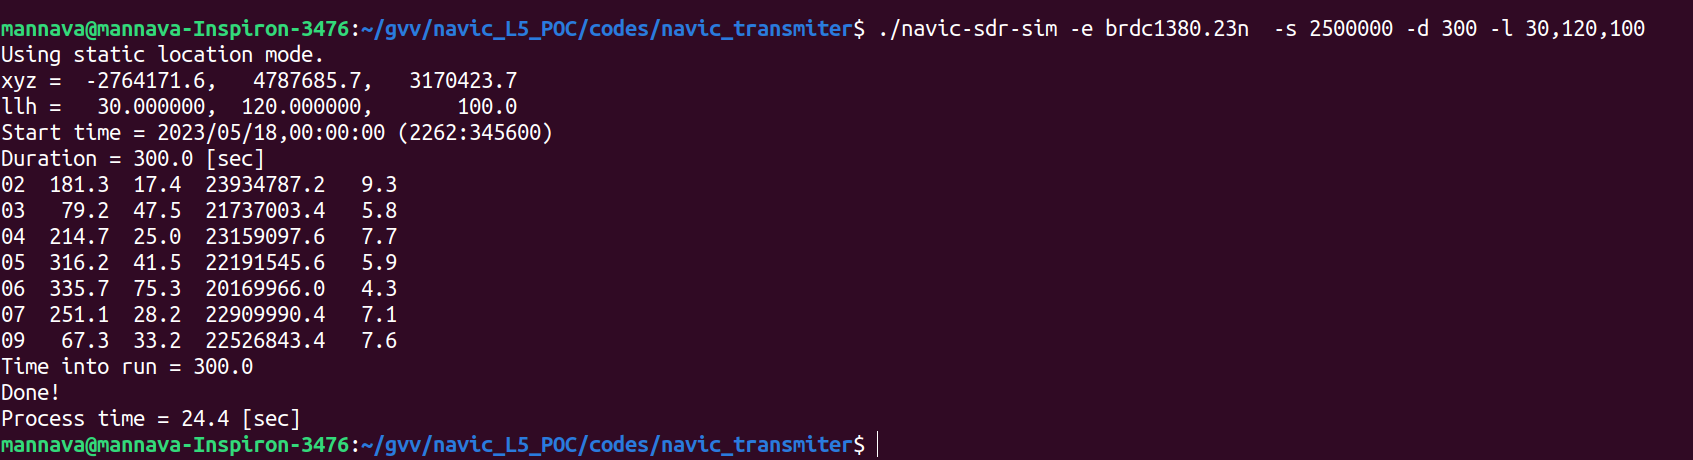
\includegraphics[width=1.25\textwidth]{figs/bin_file_gen.png}
            \centering
            \captionsetup{justification=centering}
            \caption{Generating the bin file}
            \end{figure}
        \end{normalsize}
    \item The file generated as output is 
    \begin{lstlisting}
        gvv/navic_L5_POC/codes/navic_transmiter/navicsim.bin
    \end{lstlisting}
    \item The bin file contains the IQ samples with 16 bits size. 
\end{enumerate}

\section{Transmitter frontend implementations}

\subsection{Requirements}
\begin{enumerate}
    \item The front end used at the transmitter is \textbf{USRP SDR} (Software Defined Radio).
    \item The OS used is ubuntu 22.04 version.
    \begin{normalsize}
    \begin{figure}[ht]
        \centering
        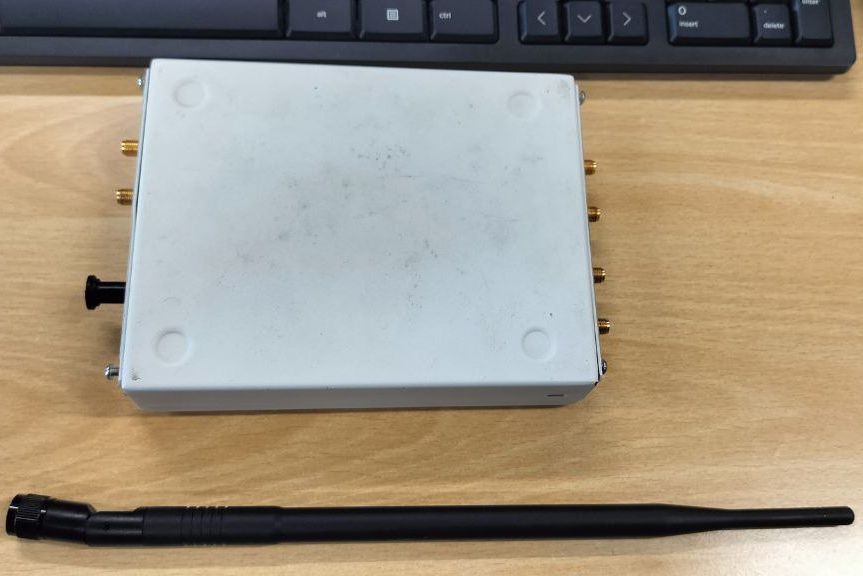
\includegraphics[width=1\textwidth]{figs/usrp.png}
        \centering
        \captionsetup{justification=centering}
        \caption{USRP SDR}
        \end{figure}
    \end{normalsize}
\end{enumerate}
\subsection*{Instalations for USRP SDR}
\begin{enumerate}
\item Install the basic requirements from the below commands. 

\begin{lstlisting}
sudo apt-get install libuhd-dev uhd-host
sudo add-apt-repository ppa:ettusresearch/uhd
sudo apt-get update
sudo apt-get install libuhd-dev uhd-host  
sudo apt-get install autoconf automake build-essential ccache cmake cpufrequtils doxygen ethtool \
g++ git inetutils-tools libboost-all-dev libncurses5 libncurses5-dev libusb-1.0-0 libusb-1.0-0-dev \
libusb-dev python3-dev python3-mako python3-numpy python3-requests python3-scipy python3-setuptools \
python3-ruamel.yaml
\end{lstlisting}
\item Clone the below repo for using the USRP and build the project.
\begin{lstlisting}
git clone https://github.com/EttusResearch/uhd.git
cd uhd/host
mkdir build
cd build
cmake ../
cmake -DCMAKE_INSTALL_PREFIX=/opt/uhd ../
make
sudo ldconfig
#run the python code 
Linux: /usr/local/lib/uhd/utils/uhd_images_downloader.py
\end{lstlisting}

\end{enumerate}

\subsection{Transmit the NavIC L5 real time samples using the Transmitter module and Transmitter frontend}

\begin{enumerate}
    \item The generated bin file in transmitter module has to be give input to the USRP so it will up convert the samples to L5 frequency and transmit the signals to air through antenna.
    \item Before feeding the bin file first we need to setup the usrp.
    \item Connect the antenna  to the USRP SDR in RF A slot in Tx/Rx port.
    \begin{normalsize}
        \begin{figure}[ht]
        \centering
        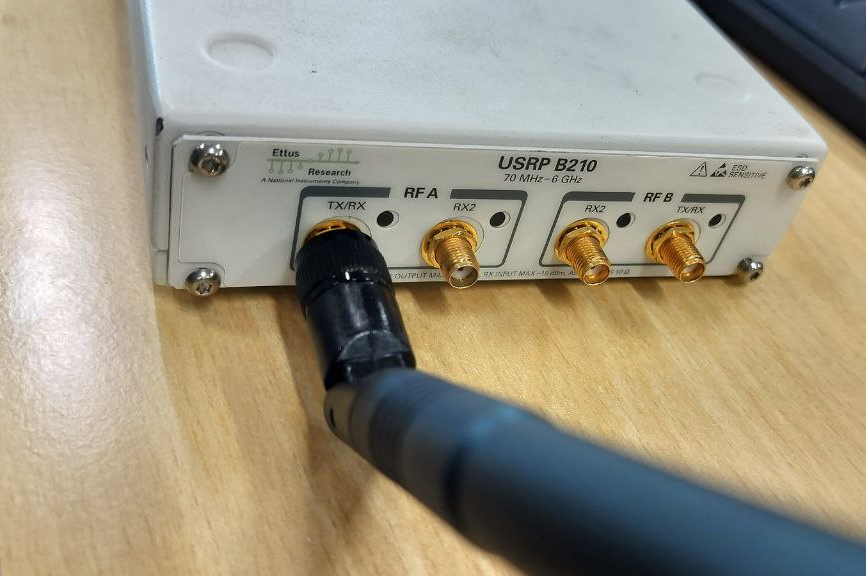
\includegraphics[width=1\textwidth]{figs/usrp_antenna.png}
        \centering
        \captionsetup{justification=centering}
        \caption{Connecting antenna to USRP SDR}
        \end{figure}
    \end{normalsize}
    \item Connect the USRP to the PC with the USB cable so that the USRP will on.
    \begin{normalsize}
    \begin{figure}[ht]
        \centering
        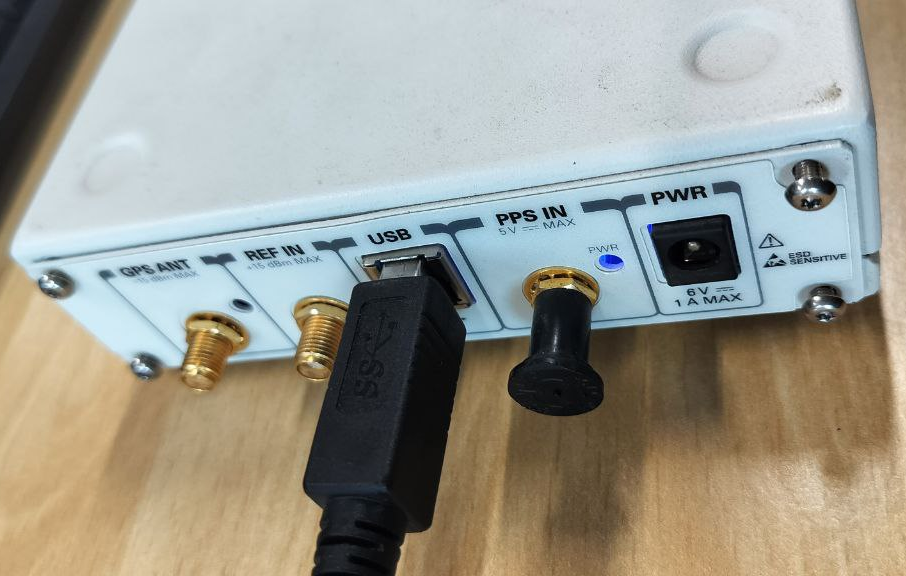
\includegraphics[width=1\textwidth]{figs/usrp_usb.png}
        \centering
        \captionsetup{justification=centering}
        \caption{Connecting USRP SDR to PC}
        \end{figure}
    \end{normalsize}
    \item Go the to uhd directory which was cloned before.
    \item In order to start the USRP use the command below.
    \begin{lstlisting}
        uhd_usrp_probe
    \end{lstlisting}
    \begin{normalsize}
    \begin{figure}[ht]
        \centering
        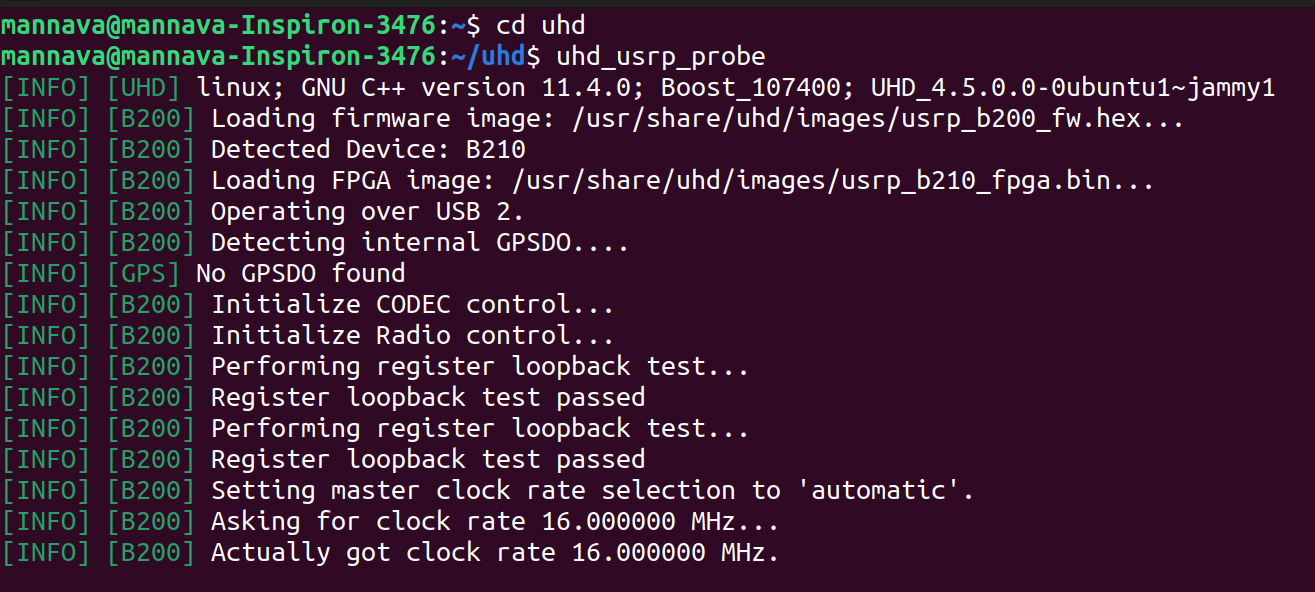
\includegraphics[width=1\textwidth]{figs/usrp_probe.png}
        \centering
        \captionsetup{justification=centering}
        \caption{Setting up the USRP SDR}
        \end{figure}
    \end{normalsize}
    \item[]
    \item Go to the below directory in uhd copy the executable file and paste in the folder that contain the bin file generated by the transmitter module.
    \begin{lstlisting}
        cd /home/mannava/uhd/host/build/examples
        cp /home/mannava/uhd/host/build/examples/tx_samples_from_file          /home/mannava/gvv/navic_L5_POC/codes/navic_transmiter

    \end{lstlisting}
    \item Run the executable file with the below command so that the bin file will feed to the USRP and USRP start transmit the signal through antenna.
    \item[]
    \item[]
    \begin{lstlisting}
        ./tx_samples_from_file --file navicsim.bin --type short --rate 2500000 --freq 1176450000 --gain 75
    \end{lstlisting}
    \item By running the command the USRP will start the transmit the signals to air.
    \item While transmiting the red led will on in usrp beside antenna port that indicate the signal is being transmiting to air through antenna.
    \begin{normalsize}
        \begin{figure}[!ht]
            \centering
            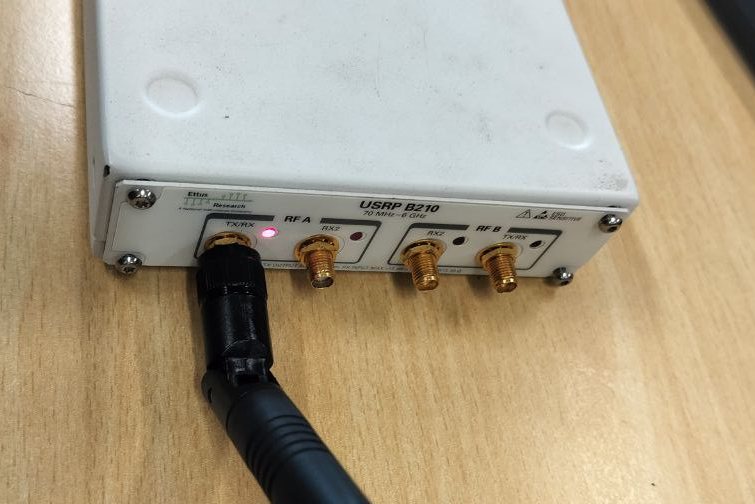
\includegraphics[width=0.7\textwidth]{figs/usrp_transmit.png}
            \centering
            \captionsetup{justification=centering}
            \caption{Signal is transmitting to air}
            \end{figure}
        \end{normalsize}
    
\end{enumerate}


\section{Receiver implementaion}

\subsection{Receiver frontend}
\begin{enumerate}
    \item The frontend used at receiver for receiving the transmitted samples and convert transmitted samples to the basband samples is \textbf{blade rf}.
    \item The OS used for implementing the receiver module is ubuntu 22.04.
    \begin{normalsize}
        \begin{figure}[!ht]
            \centering
            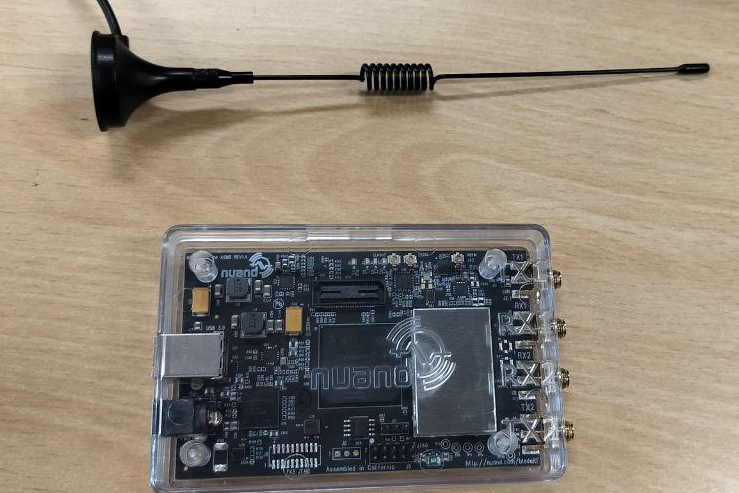
\includegraphics[width=0.6\textwidth]{figs/bladerf.png}
            \centering
            \captionsetup{justification=centering}
            \caption{Bladerf}
            \end{figure}
        \end{normalsize}
    
\end{enumerate}
\subsection{Installation for blade rf}
\begin{enumerate}
    \item Install the basic installations by the below commands.
\begin{lstlisting}
sudo add-apt-repository ppa:nuandllc/bladerf
sudo apt-get update
sudo apt-get install bladerf
sudo apt-get install libbladerf-dev
sudo apt-get install bladerf-firmware-fx3  
sudo apt-get install bladerf-fpga-hostedx40
sudo apt-get install bladerf-fpga-hostedx115
sudo apt-get install bladerf-fpga-hostedxa4
sudo apt-get install bladerf-fpga-hostedxa9

sudo apt-get install libusb-1.0-0-dev libusb-1.0-0 build-essential cmake libncurses5-dev libtecla1 libtecla-dev pkg-config git wget

dpkg -s libusb-1.0-0 libusb-1.0-0-dev
sudo apt-get install doxygen help2man pandoc
\end{lstlisting}

\item Clone the below repo and build the repo for setting up the bladerrf.
\begin{lstlisting}
git clone https://github.com/Nuand/bladeRF.git ./bladeRF
cd ./bladeRF
cd host/
mkdir build
cd build
cmake -DCMAKE_BUILD_TYPE=Release -DCMAKE_INSTALL_PREFIX=/usr/local -DINSTALL_UDEV_RULES=ON ../
groups
sudo groupadd bladerf
sudo usermod -a -G bladerf jon
make && sudo make install && sudo ldconfig
\end{lstlisting}
\end{enumerate}

\subsection{Setting up the NavIC receiver}
\begin{enumerate}
    \item The transmitted signals are received to the bladerf.The bladerf will convert the signals to baseband by removing the carrier as we discussed above chapter.These baseband samples are I and Q samples.
    \item The IQ samples are feeded to the receiver module.
    \item The receiver module perform
    \begin{enumerate}
        \item Acquisition
        \item Tracking
        \item bit synchronisation
        \item BPSK demodulation
        \item Frame synchronisation
        \item Convolutional decoding
        \item Frame decoding.
    \end{enumerate}
    \item The receiver module will perform all the above operations and gives the output as .nav file and .obs file.
    \item The nav file contains the orbital parameters of all visible satellites. From the nav file we can find the position of satellite in orbit.
    \item The obs file contains the code and carrier properties.
    \item With the nav file and obs file we can find out the position of receiver.
    \item In order to compute the location of the receiver from the nav file and obs file we use the library called RTKLIB.
    \item Clone the RTKLIB from the below repo.
    \begin{lstlisting}
        git clone git clone https://github.com/tomojitakasu/RTKLIB.git
    \end{lstlisting}
    \item Build the RTKLIB library.
    \begin{lstlisting}
        cd RTKLIB/app/rnx2rtkp/gcc
        make
    \end{lstlisting}
    \item For setting the receiver clone the below repo.
    \begin{lstlisting}
        gvv/navic_L5_POC/codes/navic_receiver
    \end{lstlisting}
    The souce codes for all the receiver module is there in below directory.
    \begin{lstlisting}
        gvv/navic_L5_POC/codes/navic_receiver/src
    \end{lstlisting}
    \item Build the project by using the make in the below directory.
    \begin{lstlisting}
        cd gvv/navic_L5_POC/codes/navic_receiver/cli/linux
        make
    \end{lstlisting}
    \item By building the project the executable file of the receiver module will be generated.
    \item The executable generated in RTKLIB is copied and paste in the below directory.
    \begin{lstlisting}
        cp /home/mannava/RTKLIB/app/rnx2rtkp/gcc/rnx2rtkp   /home/mannava/gvv/navic_L5_POC/codes/navic_receiver/bin/rinex
    \end{lstlisting}
\end{enumerate}


\subsection{Receive the signals and compute the position of receiver}
\begin{enumerate}
    \item After all the installations of bladerf and setting up the receiver module Connect the antenna to the bladerf in RX1 port.
    \begin{normalsize}
        \begin{figure}[!ht]
            \centering
            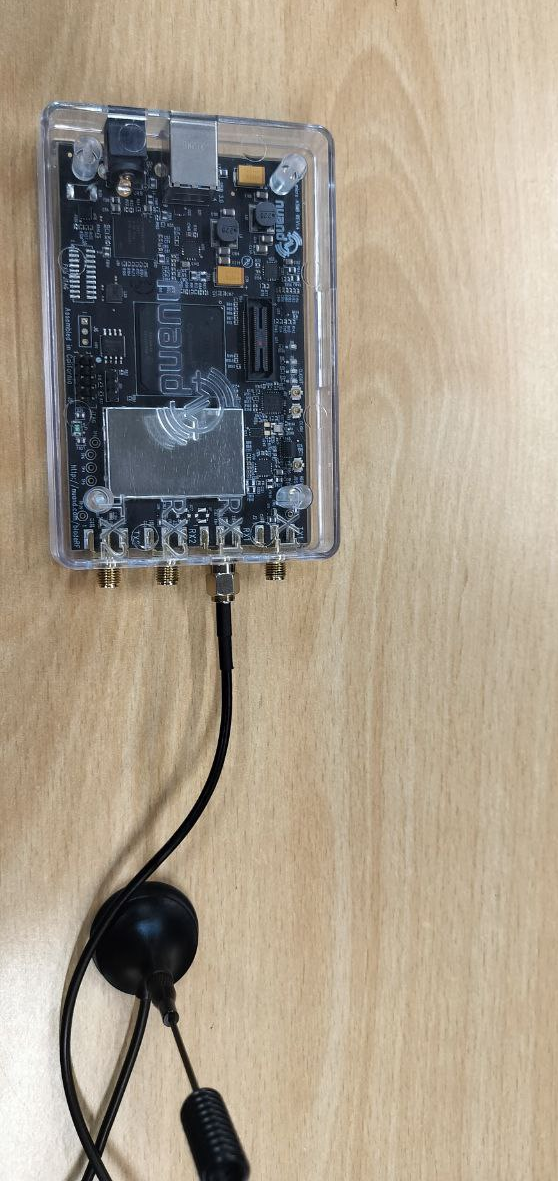
\includegraphics[width=0.4\textwidth]{figs/bladerf_antenna.png}
            \centering
            \captionsetup{justification=centering}
            \caption{Connect antenna to Bladerf}
            \end{figure}
        \end{normalsize}
    \item Connect the bladerf to the PC through the USB cable.
    \begin{normalsize}
        \begin{figure}[!ht]
            \centering
            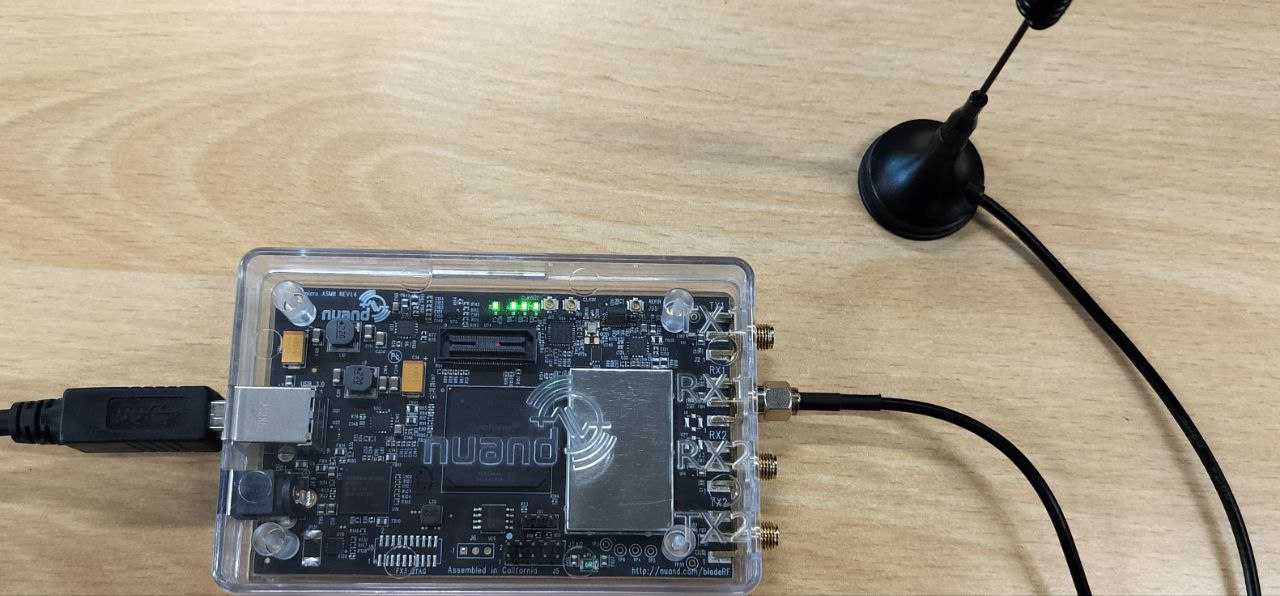
\includegraphics[width=1\textwidth]{figs/bladerf_USB.png}
            \centering
            \captionsetup{justification=centering}
            \caption{Connect Bladerf to PC}
            \end{figure}
        \end{normalsize}
    \item configure the bladerf with the center frequency,sampling frequency gain and other properties by below comands.
    \begin{lstlisting}
        bladeRF-cli -i <<EOF
        set frequency rx 1176.45e6
        set frequency tx 47e6
        set agc off
        set samplerate 2.048e6
        set bandwidth 3.0e6
        set gain rx 60
        set gain tx 0
        set clock_sel onboard
        set biastee rx off
    \end{lstlisting}
    \begin{normalsize}
        \begin{figure}[!ht]
            \centering
            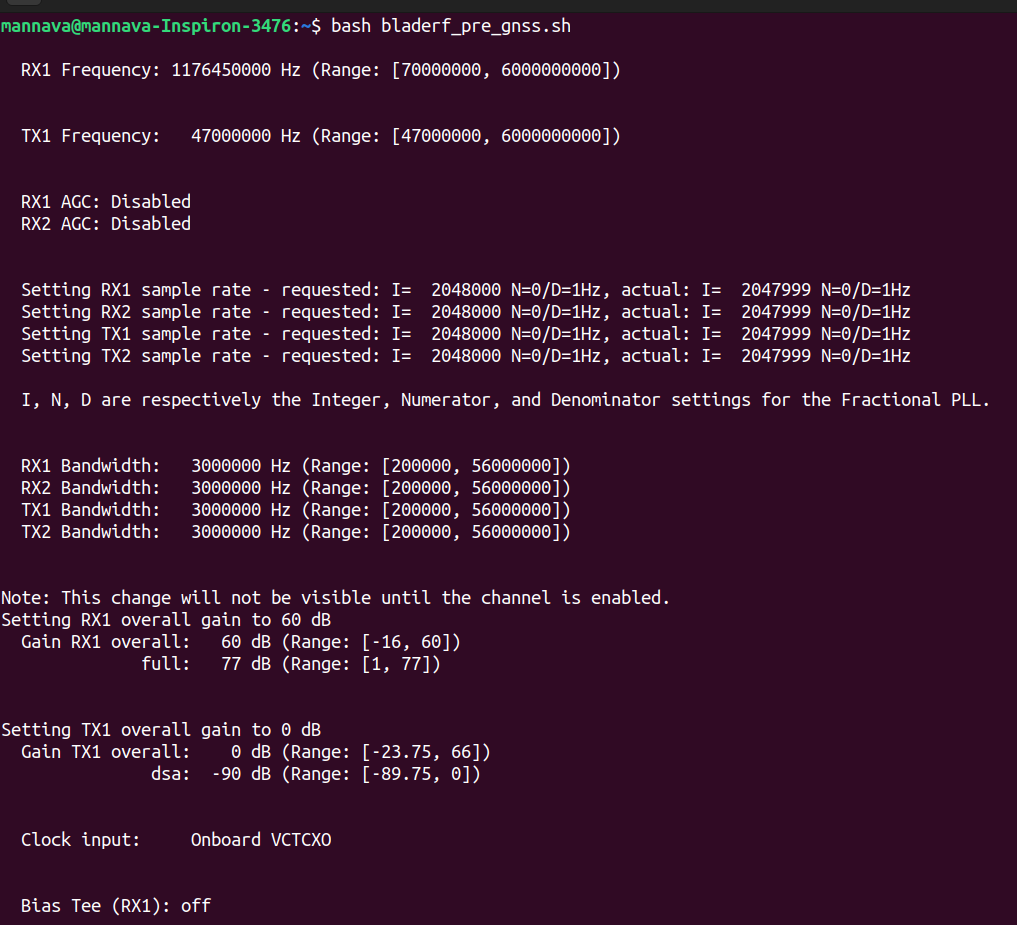
\includegraphics[width=1\textwidth]{figs/bladerf_conf.png}
            \centering
            \captionsetup{justification=centering}
            \caption{Configuring the bladerf}
            \end{figure}
        \end{normalsize}

        \item After all the configurations run the receiver module with the executable file as we generated earlier with the below command.By running the command the receiver module starts and perform all the operations of receiver and give the nav and obs files.
        \item[]
        \item[]
        \begin{lstlisting}
           cd /home/mannava/gvv/navic_L5_POC/codes/navic_receiver/bin
           ./ignss-sdrcli
        \end{lstlisting}
        \begin{normalsize}
            \begin{figure}[!ht]
                \centering
                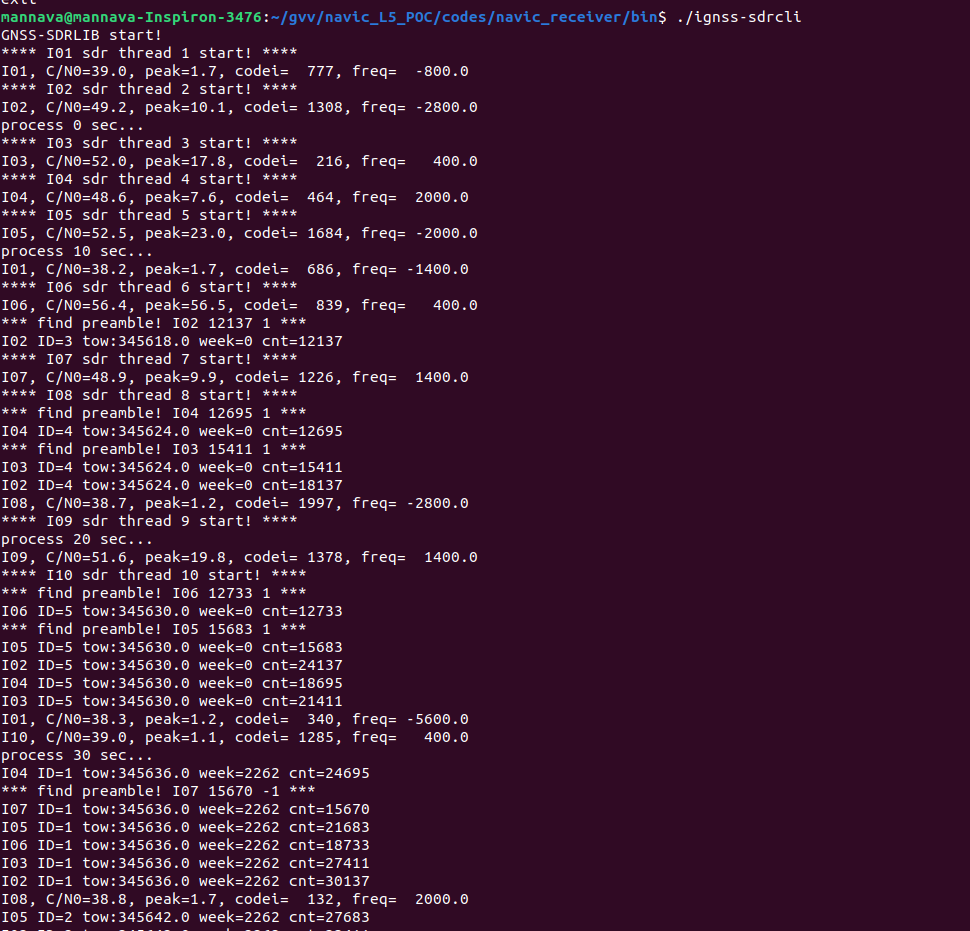
\includegraphics[width=1\textwidth]{figs/rx_execute.png}
                \centering
                \captionsetup{justification=centering}
                \caption{Output of receiver module}
                \end{figure}
            \end{normalsize}
        \item After running the receiver module the obs file and nav file are the output and stored in rinex directory.For computing the position of receiver use the following command.
        \begin{lstlisting}
            cd /home/mannava/gvv/navic_L5_POC/codes/navic_receiver/bin/rinex
            ./rnx2rtkp -p 2 -f 1 -t -s , -l 0.0 0.0 0.0  ignss-sdrlib.obs   ignss-sdrlib.nav 
         \end{lstlisting}
         \item By running the above command we get the PVT of the receiver.
         \begin{normalsize}
            \begin{figure}[!ht]
                \centering
                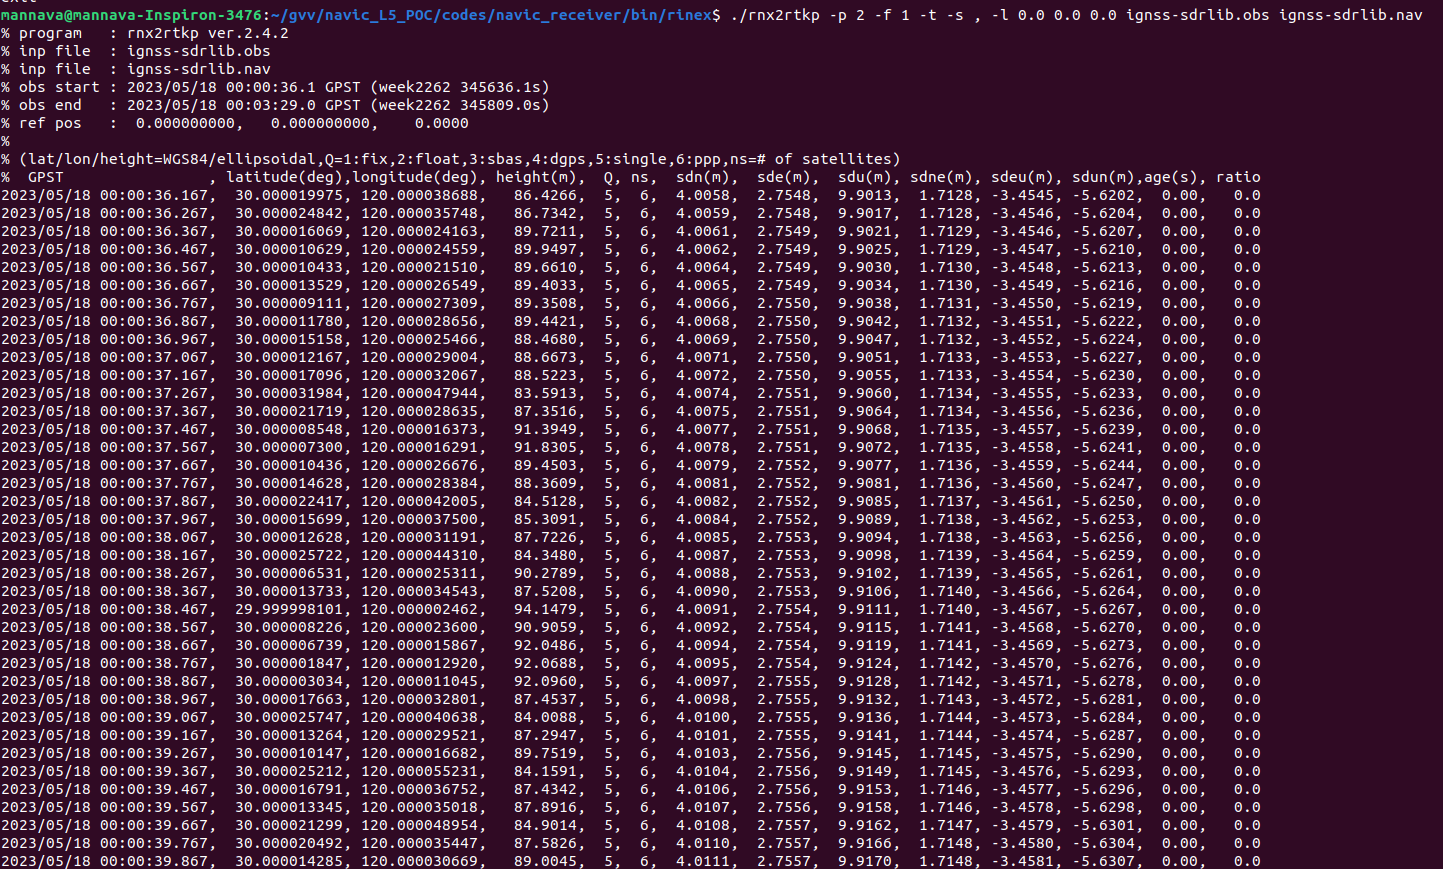
\includegraphics[width=1\textwidth]{figs/pvt.png}
                \centering
                \captionsetup{justification=centering}
                \caption{PVT of the receiver}
                \end{figure}
            \end{normalsize}

            \begin{normalsize}
                \begin{figure}[!ht]
                    \centering
                    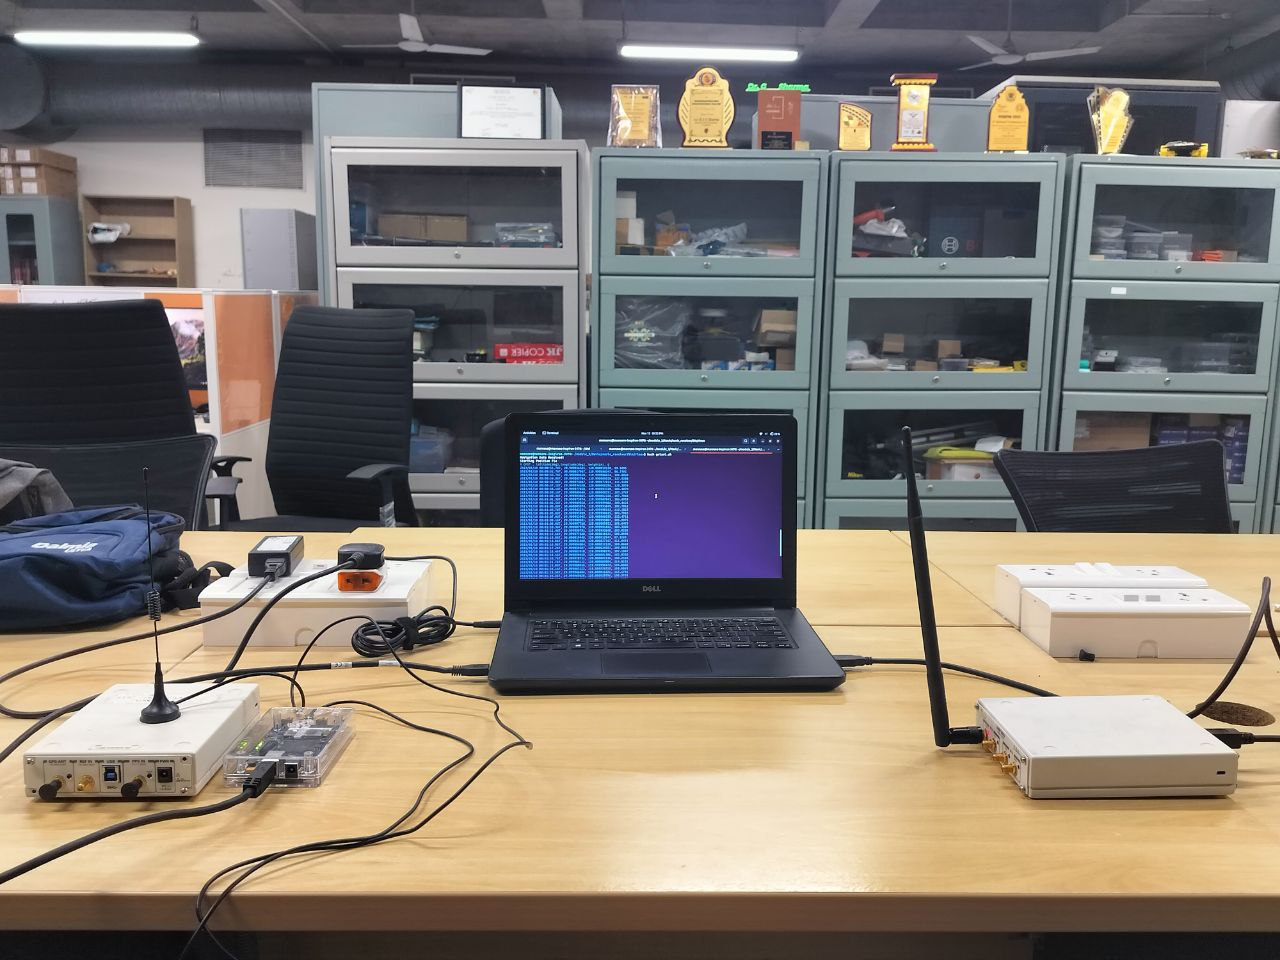
\includegraphics[width=1.2\textwidth]{figs/final.png}
                    \centering
                    \captionsetup{justification=centering}
                    \caption{final setup}
                    \end{figure}
                \end{normalsize}
\end{enumerate}








\backmatter
\appendix
\chapter{References}
\begin{enumerate}

	\item https://www.isro.gov.in/media\_isro/pdf/Publications/Vispdf/Pdf2017/\\1a\_messgingicd\_receiver\_incois\_approved\_ver\_1.2.pdf

	\item https://gnss-sdr.org/docs/sp-blocks/acquisition/

	\item https://gnss-sdr.org/docs/sp-blocks/tracking/
   
	\item Elliott D. Kaplan and Christopher J. Hegarty,  Understanding {GPS} {P}rinciples and {A}pplications, $3^{rd}$ edition
\end{enumerate}
\let\cleardoublepage\clearpage  %to remove blank page

%\newpage
%\begin{thebibliography}{00}
%\bibitem{b1} \text{https://www.isro.gov.in/media_isro/pdf/Publications/Vispdf/Pdf2017/1a_messgingicd_receiver_incois_approved_ver_1.2.pdf} 
%\bibitem{b2} \text{https://gnss-sdr.org/docs/sp-blocks/acquisition/}
%\bibitem{b3} \text{https://gnss-sdr.org/docs/sp-blocks/tracking/}
%\bibitem{b4} Elliott D. Kaplan and Christopher J. Hegarty "Understanding GPS Principles and Applications"
%\end{thebibliography}

\latexprintindex
\end{document} 
